%AMRITA UNIVERSITY PH.D latex template...Created by Chungath, CYS-CBE%
% Adapted for the B.Tech thesis "Katalyze: An Autonomous Testing Agent for Functional Bugs in Web Applications". Build: pdflatex mythesis; bibtex mythesis; pdflatex mythesis (x2).

\documentclass[a4paper, 12pt]{report}
%\renewcommand{\bibname}{References}
\usepackage[margin=0.8in]{geometry}

\usepackage{bold-extra}
\usepackage{amsmath}
\usepackage{amsfonts}
\usepackage{amssymb}
\usepackage{graphicx}
\usepackage [english]{babel}
\usepackage [autostyle, english = american]{csquotes}
\MakeOuterQuote{"}
\usepackage{setspace}
\onehalfspacing
\graphicspath{{images/}}
\usepackage{amsthm}
\usepackage{array}
\usepackage{cite}
\usepackage{longtable}
\usepackage{fancyhdr}
\usepackage{titletoc}
% Added for this thesis: tables, colour, diagrams, code paths.
\usepackage{booktabs}
\usepackage{tabularx}
\usepackage{multirow}
\usepackage{xcolor}
\usepackage{tikz}
\usetikzlibrary{arrows.meta, positioning, fit, shapes.geometric}
\usepackage{url}
\usepackage{enumitem}
\usepackage{float}
\usepackage[T1]{fontenc}
\usepackage{lmodern}
\usepackage{microtype}
\emergencystretch=2em
\theoremstyle{definition}
\newtheorem{Definition}{Definition}[section]

% Marks text that is written after tuning round v3 and the external evaluation.
\newcommand{\pending}[1]{\textcolor{red}{\textbf{[PENDING:} #1\textbf{]}}}
% Code identifiers (arm names, modules).
\newcommand{\code}[1]{\texttt{\small #1}}

%-------------------------------------------------------------
% title page
\begin{document}
	\pagenumbering{gobble}
	\thispagestyle{empty}
	\begin{large}
		\begin{center}
			{\Large\bfseries{KATALYZE: AN AUTONOMOUS TESTING AGENT FOR FUNCTIONAL BUGS IN WEB APPLICATIONS}}\\
			\vspace{1.3cm}
			A Thesis \\
			\vspace{.1cm}
			Submitted in partial fulfilment for the Degree of\\
			\vspace{.1cm}
			BACHELOR OF TECHNOLOGY\\
			\vspace{.1cm}
            in
            \vspace{.1cm}
            \\ COMPUTER SCIENCE AND ENGINEERING (ARTIFICIAL INTELLIGENCE) \\
			\vspace{1cm}
			by\\ \vspace{0.2cm}
			\vspace{.1cm}
            {\Large\bfseries{ARUNODAY A K (CB.SC.U4AIE23106)}} \\
            {\Large\bfseries{ACHUTHARAJ R (CB.SC.U4AIE23108)}} \\
            {\Large\bfseries{LOKESH D (CB.SC.U4AIE23123)}} \\
            {\Large\bfseries{ABHAY ROHIT M (CB.SC.U4AIE23173)}} \\
            \vspace{3cm}

			
\includegraphics[scale=0.8]{univA.png}\\
			\vfill
			DEPARTMENT OF ARTIFICIAL INTELLIGENCE\\
			\Large{\textbf{AMRITA VISHWA VIDYAPEETHAM}}\\
			{\large COIMBATORE CAMPUS (INDIA)}\\
			\vspace*{.3cm}
			October 2026
		\end{center}
	\end{large}
	%------------------------------------------------------------------------------------
	% bonafide certificate
	\newpage
	\begin{center}

		{\large DEPARTMENT OF ARTIFICIAL INTELLIGENCE}\\
		\Large{ \textbf{AMRITA VISHWA VIDYAPEETHAM}}\\
			{\large COIMBATORE CAMPUS}\\
		\vspace*{2.2cm}
		
\includegraphics[scale=0.8]{univA.png}\\
		\vspace*{1.5cm}
		{\Large \textbf{BONAFIDE CERTIFICATE}}
	\end{center}
	\vspace*{.8cm}
	\noindent This is to certify that the thesis entitled \enquote{\textbf{Katalyze: An Autonomous Testing Agent for Functional Bugs in Web Applications}} submitted by \textbf{Arunoday A K, Roll. No: CB.SC.U4AIE23106}, \textbf{Achutharaj R, Roll. No: CB.SC.U4AIE23108}, \textbf{Lokesh D, Roll. No: CB.SC.U4AIE23123} and \textbf{Abhay Rohit M, Roll. No: CB.SC.U4AIE23173} for the award of the \textbf{Degree of Bachelor of Technology} under the \textbf{Faculty of Engineering} is a bonafide record of the work carried out by them under my guidance and supervision at \enquote{Department of Artificial Intelligence}, Amrita Vishwa Vidyapeetham, Coimbatore Campus.\\
    \vfill
    Submitted for the examination held on .........
    \vfill
    \textbf{INTERNAL EXAMINER}    \hspace{5cm}      \textbf{EXTERNAL EXAMINER}
    \vfill
\begin{center}
		\textbf{Dr. Palmani}\\
	Thesis Advisor,\\
	Assistant Professor (Sr. Gd.),\\
	Center for Computational Engineering and Networking,\\
	School of Artificial Intelligence,\\
	Amrita Vishwa Vidyapeetham,\\
	Coimbatore Campus,\\
	India.
\end{center}

	%-------------------------------------------------------------------------------
	% Declaration page
	\newpage
	\begin{center}
	{\large DEPARTMENT OF ARTIFICIAL INTELLIGENCE}\\
	\Large{ \textbf{AMRITA VISHWA VIDYAPEETHAM}}\\

	{\large COIMBATORE CAMPUS}\\


		\vspace*{2.5cm}
		\large {\textbf{DECLARATION}}
		\vspace*{.3cm}
	\end{center}

	\noindent We,\textbf{ Arunoday A K},  \textbf{Reg. No: CB.SC.U4AIE23106}, \textbf{ Achutharaj R},  \textbf{Reg. No: CB.SC.U4AIE23108}, \textbf{ Lokesh D},  \textbf{Reg. No: CB.SC.U4AIE23123} and \textbf{ Abhay Rohit M},  \textbf{Reg. No: CB.SC.U4AIE23173} hereby declare that this thesis entitled \enquote{\textbf{Katalyze: An Autonomous Testing Agent for Functional Bugs in Web Applications}} is the record of the original work done by us under the guidance of \textbf{Dr. Palmani}, Assistant Professor (Sr. Gd.), Center for Computational Engineering and Networking, School of Artificial Intelligence, Amrita Vishwa Vidyapeetham, Coimbatore Campus. To the best of our knowledge, this work has not formed the basis for the award of any degree/diploma/associateship/fellowship or a similar award to any candidate in any University.\\\\

	\vspace*{1cm}
	\noindent{\bf Place:\hfill Signature of the Students} \\
	\noindent {\bf Date: }
	\vfill
	\begin{center}
		\large{COUNTERSIGNED}\\
	\end{center}
	\vspace{0.6in}

\begin{center}
		\textbf{Dr. K.P Soman}\\
	Professor and Dean, \\
	Department of Artificial Intelligence \\ Amrita Vishwa Vidyapeetham,\\
	Coimbatore Campus,\\
	India.
\end{center}

	%-----------------------------------------------------------------------------
	\clearpage
	\pagenumbering{roman}
	\tableofcontents

	\chapter*{Acknowledgements}
	\addcontentsline{toc}{chapter}{Acknowledgements}
	We thank our thesis advisor, Dr. Palmani, for the guidance given throughout this
project, for questioning our results whenever they looked too good, and for pushing us to state
our limitations openly. We thank Dr. K.P. Soman, Professor and Dean, and the faculty of the
Department of Artificial Intelligence for the facilities and the review process that shaped
this work. We are grateful to the researchers who made their web-testing subject applications
public: the authors of WebExplor and WebRLED, and Matteo Biagiola and colleagues, whose
replication material packages those applications with their instrumentation. Without open
benchmarks, an honest comparison with published work would not be possible. Finally, we thank
our families and friends for their support.\\
	\vspace{1cm}
	\begin{flushright}
		ARUNODAY A K \\
		ACHUTHARAJ R \\
		LOKESH D \\
		ABHAY ROHIT M
	\end{flushright}
	\listoffigures
	\addcontentsline{toc}{chapter}{List of figures}
	\listoftables
	\addcontentsline{toc}{chapter}{List of tables}
	\newpage
\section*{{\huge Abbreviations}\hfill} \addcontentsline{toc}{chapter}{\textbf{Abbreviations}}
\vspace{1.2cm}
\begin{tabular}{lll}
AC-DQN ~~~~&--&~~~~ Action-Conditioned Deep Q-Network\\
AUROC ~~~~&--&~~~~ Area Under the Receiver Operating Characteristic curve\\
CRUD ~~~~&--&~~~~ Create, Read, Update, Delete\\
DOM ~~~~&--&~~~~ Document Object Model\\
DQN ~~~~&--&~~~~ Deep Q-Network\\
GUI ~~~~&--&~~~~ Graphical User Interface\\
LLM ~~~~&--&~~~~ Large Language Model\\
MDP ~~~~&--&~~~~ Markov Decision Process\\
PER ~~~~&--&~~~~ Prioritised Experience Replay\\
RL ~~~~&--&~~~~ Reinforcement Learning\\
RMST ~~~~&--&~~~~ Restricted Mean Survival Time\\
SPA ~~~~&--&~~~~ Single-Page Application\\
UI ~~~~&--&~~~~ User Interface\\
\end{tabular}
\newpage
\section*{{\huge List of symbols}\hfill} \addcontentsline{toc}{chapter}{\textbf{List of symbols}}
\vspace{1.2cm}
\begin{tabular}{lll}
$s, s'$ ~~~~&--&~~~~ State before and after an action\\
$a$ ~~~~&--&~~~~ Action (one browser interaction)\\
$\phi(a)$ ~~~~&--&~~~~ Feature vector describing action $a$\\
$Q(s, \phi(a))$ ~~~~&--&~~~~ Action-conditioned action value\\
$\gamma$ ~~~~&--&~~~~ Discount factor\\
$\epsilon$ ~~~~&--&~~~~ Exploration rate\\
$\Phi(s)$ ~~~~&--&~~~~ LLM-assessed task progress of state $s$, in $[0,1]$\\
$\lambda$ ~~~~&--&~~~~ Weight of the LLM reward term\\
$B$ ~~~~&--&~~~~ Interaction budget of one run (2{,}000)\\
$T$ ~~~~&--&~~~~ Interactions to the first verified fault ($T=B$ if none)\\
$\mathrm{Beta}(\alpha, \beta)$ ~~~~&--&~~~~ Beta posterior of a bandit key\\
$N(s, a, s')$ ~~~~&--&~~~~ Visit count of a page transition\\
\end{tabular}
\chapter*{Abstract}
\addcontentsline{toc}{chapter}{Abstract}
Web applications fail in ways that are easy to describe and hard to find: a total that
ignores a changed quantity, a validation rule that holds on one path and not on another, a
value that is lost on reload. Automated exploratory testers can reach such states, but they
face two problems. They must decide where to go in a large, stateful interface where the
decisive actions are many steps deep, and they must prove what they find, or their reports
are noise. This thesis builds and evaluates \emph{Katalyze}, an automated functional
tester for web applications that uses reinforcement learning (RL). It confirms a fault only when the fault
reproduces twice in fresh browser sessions, is absent from a control build without that
fault, and survives delta-debugging minimisation.

The work has two generations. The first (v1) is an action-conditioned dueling double deep
Q-network that scores every available browser action, with prioritised multi-step replay, a
residual head for online adaptation, and a reward shaped by a local large language model
(LLM) that judges task progress. Two pre-registered experiments tested it. Pretraining on
five applications did not speed up fault discovery on a sixth (median difference 0
interactions, 95\% interval $[-749, +290]$). A diagnostic over twelve generated application
variants found that the network does not learn which action helps in which state
(within-label AUROC 0.51). Post-hoc checks showed that the LLM's progress score and its page
labels did not generalise beyond the data they were tuned on.

These findings shaped the second generation (v2), a hybrid tester. It abstracts pages
explicitly, keeps an archive of reached states that it returns to by exact replay
(Go-Explore), and applies test operators from standard test design. A light online learner
(a Thompson-sampling bandit, or count-based curiosity Q-learning) decides which operator to
try. On eight held-out applications, in a pre-registered evaluation of 160 runs with 32
clean-build controls, the hybrid arms verified the most distinct faults (19 and 18 of 24,
against 13 for random exploration) with zero false positives. All four pre-registered
comparisons of time to first fault were inconclusive.
After re-tuning on rebuilt full-stack development applications, the frozen tester was
compared with WebExplor and WebRLED on their six subject applications, measured as they were
measured: one-hour runs, Istanbul branch coverage and console failures. It did not reach
their published numbers. It averaged 44.3\% branch coverage against 55.5\% and 64.2\%, and
1.8 distinct console failures against 3.1 and 4.1. A post-hoc follow-up traced much of the
gap to the tester's action space rather than its policy. With clickable elements that plain
HTML scanning misses, coverage on Phoenix rose from 49\% to 83\% for every arm, level with
WebRLED. The evidence supports
a modest conclusion: the structure of a tester, more than the learning in it, determines
which functional faults it verifies.

\vspace{0.5cm}
\noindent\textbf{Keywords:} automated web testing, reinforcement learning, deep Q-network,
Go-Explore, Thompson sampling, test oracle, seeded faults, survival analysis.


\clearpage
\pagenumbering{arabic}
\setcounter{page}{1}
\chapter{Introduction}
\label{chap.1}

\section{Motivation}

Web applications carry much of everyday business: shops, banking, booking, support desks,
internal tools. Their functional faults are rarely crashes. More often a page shows the
wrong total after a quantity changes, accepts an input on one path that it rejects on
another, or loses a value when the page is reloaded. Such faults sit behind sequences of
interactions: a user must sign in, fill a form, reach a review step, go back and change
something. A tester has to perform the right sequence and then notice that the result is
wrong.

Writing scripted end-to-end tests for every such sequence is expensive, and the scripts
cover only what their authors thought of. Automated exploratory testing instead drives a real
browser through the application and searches for misbehaviour. The simplest explorer clicks
at random. More capable explorers learn where to go, and reinforcement learning (RL) is a
natural fit: the tester is an agent, the application is its environment, and reaching new or
suspicious behaviour can be rewarded. Several RL web testers have been published, including
WebExplor~\cite{zheng2021webexplor}, WebQT~\cite{chang2023webqt} and
WebRLED~\cite{gu2025webrled}.

Two problems limit these testers. The first is \emph{where to go}. The decisive actions are
often many steps into a workflow, the set of available actions changes on every page, and a
reward based on novelty pays for reaching new pages, not for testing them. The second is
\emph{what counts as a fault}. Published RL web testers report errors in the browser console
as failures~\cite{zheng2021webexplor, gu2025webrled}. That is an implicit
oracle~\cite{barr2015oracle}: it cannot see a page that renders the wrong content without an
error, and it cannot say whether a reported error is reproducible or matters.

\section{Problem statement}

This thesis asks whether reinforcement learning can make an automated functional tester for
web applications find \emph{verified} faults sooner, and under what design. A fault is
verified when it reproduces twice in fresh browser sessions, is absent from a control build
that lacks that one fault, and survives delta-debugging minimisation~\cite{zeller2002simplifying}.
The main measure is the number of browser interactions until the first verified fault, with
runs that find nothing treated as right-censored at the budget.

\section{Objectives}

\begin{enumerate}
  \item Build a browser environment and a deterministic, replay-verified oracle for seeded
        faults that makes false positives measurable and rare.
  \item Build a deep RL tester and test, under pre-registration, whether pretraining on other
        applications transfers to a new one, and whether the network learns which action
        helps in which state.
  \item Measure whether a small, local large language model (LLM) is a useful source of
        reward or page labels for testing.
  \item Use those findings to design a tester whose exploration does not depend on what the
        deep network failed to learn, and evaluate it on held-out applications under
        pre-registration.
  \item Compare the final tester with published RL web testers on their own subject
        applications. \pending{Outcome of this objective.}
  \item Package the tester as a usable product: a command-line tool and a web interface that
        test a URL, a static site, a Dockerfile repository or a bundled application and
        produce a report with evidence.
\end{enumerate}

\section{Contributions}

\begin{enumerate}
  \item \textbf{A verified-fault oracle for web testing.} Each seeded fault has its own
        control build. A candidate counts only if it reproduces twice, does not occur on
        that control, and survives minimisation. The oracle produced zero false positives in
        every clean-build control run of every evaluation.
  \item \textbf{A pre-registered transfer experiment for deep RL web testing}, using
        leave-one-application-out evaluation and censoring-aware statistics. Its result is
        negative: pretraining gave no measurable benefit.
  \item \textbf{A pre-registered diagnostic separating contextual learning from
        memorisation.} It uses a generated application family and probe states labelled by
        execution, and shows that the v1 network does not learn context.
  \item \textbf{Two negative results for small local LLMs in testing}, each measured
        against ground truth: as a progress reward, and as a page and control labeller.
  \item \textbf{A hybrid tester} combining page abstraction, an archive with exact return,
        test operators from standard test design, and a light online learner. It was
        evaluated on eight held-out applications under pre-registration, and verified the
        most distinct faults with zero false positives.
  \item \textbf{Sixteen test applications with real backends and seeded faults}, each
        admitted by mechanical checks. The eight development applications run on PostgreSQL
        or MongoDB, with sign-in and crash-type faults.
  \item \pending{External comparison with WebExplor and WebRLED.}
\end{enumerate}

\section{Scope}

The project began with two agents: one for security testing and one for functional testing.
The security agent was dropped early so that one agent could be built and evaluated end to
end. \textbf{Security testing is out of scope}; this thesis is about functional testing.
The applications are small to medium web applications with seeded faults. Claims about
production sites or real-world fault rates are outside what the evidence supports, and
Chapter~\ref{chap.6} states the limits on generalisation.

\section{Organisation of the thesis}

Chapter~\ref{chap.2} reviews RL web and GUI testing, the deep RL and exploration methods
used here, LLM-derived rewards, test oracles and evaluation statistics.
Chapter~\ref{chap.3} describes the system around the tester: the browser environment, the
action registry, the verified-fault oracle and the product layer. Chapter~\ref{chap.4}
presents the first-generation deep RL tester and the experiments that tested it.
Chapter~\ref{chap.5} presents the hybrid tester designed from those results, and its
development rounds. Chapter~\ref{chap.6} describes the test applications and the evaluation
methodology. Chapter~\ref{chap.7} reports the evaluations. Chapter~\ref{chap.8} concludes.

\chapter{Background and Related Work}
\label{chap.2}

This chapter positions the work. Section~\ref{sec:bg-webtesting} covers automated web
testing and its oracles, Section~\ref{sec:bg-rltesting} RL for web and GUI testing,
Section~\ref{sec:bg-llm} LLM-driven testing and LLM-derived rewards,
Section~\ref{sec:bg-drl} the deep RL and exploration methods the testers are built from,
and Section~\ref{sec:bg-eval} how such tools are evaluated. Section~\ref{sec:bg-gap} states
the gap this thesis addresses. Statements about what a paper did or found are taken from its
abstract or full text; paragraphs headed \emph{For this work} are our reasoning.

\section{Automated web testing and test oracles}
\label{sec:bg-webtesting}

An automated web tester drives a browser through an application and decides, at each page,
what to do next. Crawljax established the model-based approach for
JavaScript-heavy applications: it infers a state-flow graph of user-interface states by
firing events and comparing the resulting DOM. Model-based and search-based testers explore
systematically, while random ("monkey") testers are cheap and, in GUI testing, a notoriously
strong baseline.

Exploring is only half of testing. The other half is deciding whether what happened was
wrong: the oracle problem. Barr et al.~\cite{barr2015oracle} classify oracles as specified
(a specification says what is correct), derived (from artefacts such as earlier versions),
implicit (generic failures such as crashes and exceptions) and absent (left to a human). RL
web testers use implicit oracles, namely errors in the browser console~\cite{zheng2021webexplor, gu2025webrled}. These are cheap and general, but blind to wrong content that renders without
error.

A \emph{seeded-fault oracle} is a specified oracle for a known set of faults. It provides
ground truth, which evaluation methodology in fuzzing prefers: Klees
et al.~\cite{klees2018evaluating} recommend measuring against known bugs rather than
heuristic proxies, and Magma inserts real bugs into real software with
instrumentation so that bug-centric metrics do not depend on the tool. The cost is validity.
Just et al. studied 357 real faults in five Java programs and found
mutant detection significantly correlated with real-fault detection, but 17\% of real
faults were not coupled to any mutant. Seeded faults are a supported but incomplete proxy.

Once a failure is found, delta debugging~\cite{zeller2002simplifying} minimises the failing
input while preserving the failure. Its original case study reduced 95 user actions that
crashed a browser to 3; it is used in the same way here, to shorten a reproduction trace.

\section{Reinforcement learning for web and GUI testing}
\label{sec:bg-rltesting}

\paragraph{Web.} WebExplor~\cite{zheng2021webexplor} is the reference point. It uses
curiosity-driven RL to generate action sequences, with tabular Q-learning and a curiosity
reward computed from a visit-count table over transitions, and builds an automaton online
that sends the agent back to under-explored states. Training and testing are intertwined:
the policy is learned on the application under test. Its failures are console errors, and
the authors note that this oracle may miss UI bugs. WebQT changes the
reward to encourage interaction like a human tester's and treats pages with the same
function as one state, reporting higher code coverage on seven open-source applications.
QExplore combines tabular Q-learning with a guided search and text
input generation.

WebRLED~\cite{gu2025webrled} combines a deep Q-network with a grid-based action-value
scheme, a learned action discriminator, and a curiosity reward that considers novelty both
within an episode and over the global history. Liu et al. train a DQN
or PPO agent to guide a crawler towards higher branch coverage. MARG runs
several Q-learning agents that share Q-table data; its successor
WebCQ moves to deep multi-agent RL and builds a vector for each
candidate action, concatenated with the state vector, because "the available UI events vary
across states". WebCQ is the closest architectural neighbour of this thesis's first tester.

A 2026 empirical study~\cite{liu2026webgui} compares model-based, RL-based and LLM-based
web testers under six state abstractions. No single strategy excels on every dimension;
RL-based approaches most often achieve the highest coverage; compact state abstractions suit
RL; and code coverage is only weakly correlated with the ability to reveal failures.

\paragraph{Mobile.} Q-testing uses a curiosity reward from a neural
state-comparison module. ARES reports that deep RL achieves higher
coverage and fault revelation than baselines including Q-testing.
DinoDroid~\cite{zhao2024dinodroid} is the clearest precedent for learning across
applications: a deep Q-network learns a behaviour model from a set of existing apps and is
used on new ones, evaluated by two-fold cross-validation over 64 apps (32 for training in
each fold). Humanoid~\cite{li2019humanoid} learns from human interaction traces and reports
higher coverage than six other generators, but its authors add that the learned model "was
not the main reason" for the improvement.

\paragraph{For this work.} The RL agent design is not new in itself. Count-based curiosity
is the default reward in this line of work, per-action scoring over a variable action set is
published, and pretraining on some applications to test others has been
done on Android~\cite{zhao2024dinodroid}. What differs here is the oracle (verified seeded
faults instead of console errors), the outcome measure (time to the first verified fault
instead of coverage), and the question asked of the learner (does it transfer, and does it
use context).

\section{Language models in testing and as reward}
\label{sec:bg-llm}

\paragraph{LLMs as testers.} GPTDroid frames mobile GUI testing as a
question-answering loop with an LLM. DroidAgent sets its own task
goals and pursues them, reporting 61\% activity coverage against 51\% for earlier
techniques on 15 apps. AXNav executes natural-language accessibility
tests, and VETL uses a vision-language model for text inputs and element
selection on the web, with exploration guided by a multi-armed bandit. The 2026 study
tempers this line: its LLM-based web tester completed three to four times fewer actions in
the same time budget, because every decision invokes the model, and it repeated failed or
invalid actions~\cite{liu2026webgui}. Web-navigation benchmarks show how hard it is to act
reliably on unseen sites: in WebArena the best GPT-4 agent reached
14.41\% task success against 78.24\% for humans, and on Mind2Web
step success fell from 52.0\% on unseen tasks to 38.9\% on unseen websites.

\paragraph{LLMs as reward.} Kwon et al. prompt an LLM as a proxy
reward function. ELLM rewards an agent for achieving goals an LLM suggests,
motivated by the observation that novelty bonuses help little where most novelty is
irrelevant. Motif distils LLM preferences into an intrinsic
reward; Eureka and Text2Reward have the LLM
write reward code. Vision-language models have served as success
detectors and zero-shot reward models, whose
failures trace to the model's capability limits. Klissarov et al.
find that LLMs are better used to build reward models than to act directly.

\paragraph{Shaping.} Ng, Harada and Russell prove that adding a reward
equal to the discounted difference of a potential function over successive states,
$\gamma\Phi(s') - \Phi(s)$, leaves the optimal policy unchanged.
Wiewiora shows the equivalence to initialising Q-values from the
potential, and Devlin and Kudenko extend the guarantee to
potentials that change during learning. LLM-derived potentials already exist: Lin
et al. use score differences from an LLM-trained state scorer as a
potential, and report that with weaker models a direct reward outperformed the potential
form. M\"uller and Kudenko learn the potential from preferences given
by small vision-language models.

\paragraph{For this work.} Policy invariance concerns the optimal policy. It says nothing
about behaviour within a finite budget, which is what a tester is measured on. The evidence
for LLM rewards comes from games, robotics and synthetic web tasks; none of the retrieved
works evaluates an LLM-derived reward for testing. A small, local judge is on the weak side
of the capability evidence.

\section{Deep reinforcement learning and exploration}
\label{sec:bg-drl}

\paragraph{Value-based deep RL.} Q-learning learns the value
$Q(s,a)$ of taking action $a$ in state $s$ and acting well afterwards, by bootstrapping
from the next state's value. DQN~\cite{mnih2015human}
approximates $Q$ with a neural network. Double DQN~\cite{vanhasselt2016double} reduces
DQN's overestimation by decoupling action selection from evaluation. Dueling
networks separate state value from action advantage and give better
estimates when many actions have similar values, which fits pages with many near-equivalent
links. Prioritised replay replays informative transitions more
often, and Rainbow combines six such extensions, including
multi-step targets. These components were validated mainly on Atari, and Henderson
et al. show how variance makes deep RL improvements hard to
judge.

\paragraph{Variable action sets.} A web page offers a different set of actions on every
page. Dulac-Arnold et al. embed actions in a continuous space so
that a policy can generalise over them. The deep reinforcement relevance
network~\cite{he2016drrn} embeds state and text action separately and combines them to
approximate $Q$; this is the direct ancestor of the action-conditioned network
$Q(s,\phi(a))$ used here. Jain et al. treat generalisation to
unseen actions as its own problem, needing dedicated training objectives. Sentence
embeddings from compact distilled encoders
supply action-label features.

\paragraph{Exploration.} Count-based exploration rewards rarely visited states:
pseudo-counts generalise counting to large state spaces, and
hashing-based counts work with simple hash functions, provided
the hash has the right granularity. That is the same sensitivity to state abstraction that
the web-testing study measured~\cite{liu2026webgui}. Random network
distillation derives a novelty bonus from prediction error.
Go-Explore~\cite{ecoffet2021first} attributes poor exploration to two failures: forgetting
how to reach promising states, and not returning to a state before exploring from it. It
remedies both by keeping an archive of visited states and returning to them first.

\paragraph{Bandits.} A multi-armed bandit chooses repeatedly among options with unknown
payoff. Thompson sampling~\cite{russo2018tutorial} keeps a posterior
over each option's payoff, samples from it, and picks the best sample, which balances trying
uncertain options against exploiting good ones. With a Beta posterior over a success
probability, it needs only two counts per option, so it can learn within the few dozen
decisions of a single test run.

\paragraph{Generalisation.} Cobbe et al. find that agents
overfit to surprisingly large training sets, and Procgen shows that
diverse training distributions are essential. The survey by Kirk et al.
treats the number of training contexts as a core property of an evaluation protocol and
suggests fast online adaptation as a direction. With five training applications per fold,
the literature predicts weak transfer.

\section{Evaluating testing tools}
\label{sec:bg-eval}

Arcuri and Briand found that software-engineering studies of
randomised algorithms often did not account properly for randomness, and argue for enough
runs and rigorous statistical tests. Klees et al.~\cite{klees2018evaluating} examined 32
fuzzing papers and found problems in every evaluation, recommending multiple trials,
statistical tests, ground truth and a diverse benchmark; a follow-up over 150 papers found
the guidelines still widely ignored. In deep RL, Agarwal
et al. recommend stratified-bootstrap interval estimates over
point estimates.

When a tool may not find a bug within the time allowed, time to bug is a right-censored
outcome. Survival analysis handles this: the Kaplan--Meier
estimator estimates the probability of not yet having found
the bug at each time, and the restricted mean survival time (RMST)
averages the time to event up to a horizon. Magma applies Kaplan--Meier to time to
bug, and Herrera et al. report RMST with
confidence intervals and compare with the log-rank test. None of the GUI-testing papers
reviewed uses censoring-aware analysis: WebExplor averages 15 thirty-minute runs and applies
a Mann--Whitney U test~\cite{zheng2021webexplor}.

\section{Research gap}
\label{sec:bg-gap}

Within the literature reviewed:

\begin{enumerate}
  \item \textbf{Ground-truth evaluation of RL web testers.} Web RL testers are scored on
        coverage and console errors~\cite{zheng2021webexplor, gu2025webrled}. No retrieved work evaluates a web-testing policy, or
        its transfer to held-out applications, against a deterministic oracle for seeded
        faults.
  \item \textbf{An LLM-derived reward in testing.} LLM rewards and potentials exist for games
        and control, and LLMs in GUI testing act as
        the policy. Using an LLM
        only to shape a cheap learned policy is untested.
  \item \textbf{Censoring-aware, fault-centric evaluation in GUI testing.} Time to the first
        verified fault with right-censoring imports fuzzing's method into a field that
        reports averaged coverage, which is weakly related to failure
        discovery~\cite{liu2026webgui}.
  \item \textbf{Whether learning is what helps.} Humanoid's authors found their learned model
        was not the main cause of their gain~\cite{li2019humanoid}. Separating the
        contribution of learning from that of structure needs ablations against strong
        non-learning baselines.
\end{enumerate}

The contribution of this thesis is the combination and the evaluation discipline. The agent
architecture, the curiosity reward, the archive and the LLM potential each have direct
precedents and are not claimed as novel.

\chapter{System Overview and the Verified-Fault Oracle}
\label{chap.3}

This chapter describes the parts shared by both generations of the tester: the browser
environment and its action space (Section~\ref{sec:env}), the oracle that decides what is a
fault (Section~\ref{sec:oracle}), and the product layer that turns an application into a
test run and a report (Section~\ref{sec:product}). Figure~\ref{fig:system} shows how they fit
together. The explorer in the middle is the part that differs between v1
(Chapter~\ref{chap.4}) and v2 (Chapter~\ref{chap.5}).

\begin{figure}[H]
\centering
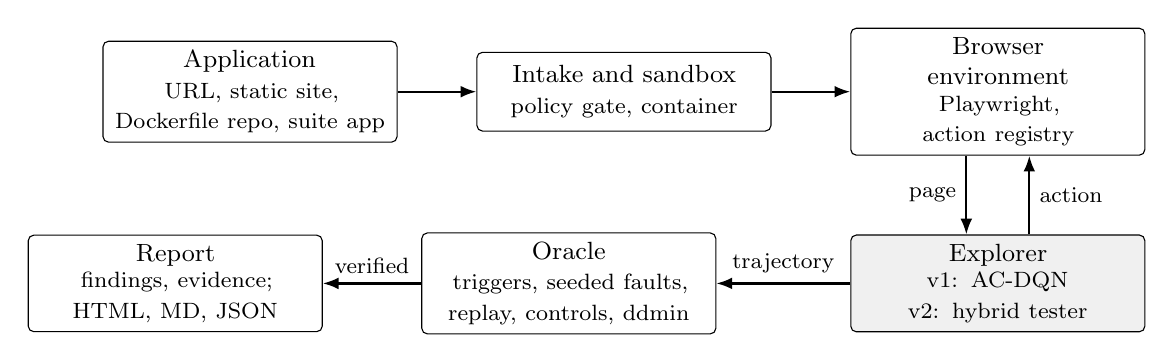
\begin{tikzpicture}[
  box/.style={draw, rounded corners=2pt, align=center, minimum height=1.0cm,
              text width=3.5cm, font=\small, execute at begin node={\hyphenpenalty=10000}},
  arr/.style={-{Latex[length=2mm]}, thick}]
  \node[box] (in) {Application\\\footnotesize URL, static site, Dockerfile repo, suite app};
  \node[box, right=1.0cm of in] (sb) {Intake and sandbox\\\footnotesize policy gate, container};
  \node[box, right=1.0cm of sb] (env) {Browser\\ environment\\\footnotesize Playwright,\\ action registry};
  \node[box, below=1.0cm of env, fill=gray!12] (ex) {Explorer\\\footnotesize v1: AC-DQN\\ v2: hybrid tester};
  \node[box, left=1.7cm of ex] (or) {Oracle\\\footnotesize triggers, seeded faults, replay, controls, ddmin};
  \node[box, left=1.25cm of or] (rep) {Report\\\footnotesize findings, evidence;\\ HTML, MD, JSON};
  \draw[arr] (in) -- (sb);
  \draw[arr] (sb) -- (env);
  \draw[arr] (env.south) ++(-0.4,0) -- ++(0,-1.0) node[midway, left, font=\footnotesize]{page};
  \draw[arr] (ex.north) ++(0.4,0) -- ++(0,1.0) node[midway, right, font=\footnotesize]{action};
  \draw[arr] (ex) -- node[above, font=\footnotesize]{trajectory} (or);
  \draw[arr] (or) -- node[above, font=\footnotesize]{verified} (rep);
\end{tikzpicture}
\caption{The system around the explorer. Only the explorer differs between v1 and v2.}
\label{fig:system}
\end{figure}

\section{The browser environment}
\label{sec:env}

The environment exposes a live application through Playwright and headless Chromium. Each
\emph{episode} starts in a fresh browser context from the application's entry page, so
cookies and local storage do not leak between episodes. For applications behind a login, a
scripted sign-in macro runs at the start of every episode; it is outside the agent's
decisions but inside the interaction budget. Server state is reset between runs, and for the
database-backed suite applications each browser context gets its own data partition
(Chapter~\ref{chap.6}).

After every action the environment waits for the page to settle. It watches the DOM with a
mutation observer and treats the page as settled after a quiet period, rather than waiting
for the network to go idle, which applications that poll or hold a websocket never
satisfy.

\subsection{Action registry}

At each step the registry scans the page and builds the set of available actions, at most
100. It combines page-independent actions (no-op, scroll, resize the viewport, browser
back, forward and refresh) with actions derived from the page's interactive elements:

\begin{itemize}[noitemsep]
  \item \textbf{click} on links, buttons and toggles, and \textbf{rapid click} (a double
        submit) on buttons;
  \item \textbf{type} into text fields, with one value from each of five categories: a
        valid typical value, the boundary minimum, the boundary maximum, an empty string,
        and a value of the wrong type;
  \item \textbf{select} an option of a dropdown;
  \item optionally, \textbf{custom clickables}: elements made interactive by ARIA roles,
        click handlers, tab index or a pointer cursor, which plain HTML scanning misses.
\end{itemize}

When a page has more candidates than slots, the budget is filled in priority order: fixed
actions, then clicks (needed to progress any flow), then valid typed values (so forms can be
submitted), then selects and rapid clicks, then the boundary and invalid variants. Elements
visible in the viewport are allocated before those below the fold. Actions are identified by
stable selectors (an element's id or name, else a structural path), so the same control
keeps its identity across visits.

\subsection{Deterministic triggers}

On every step the environment records generic failure signals: console errors, uncaught
page errors, unexpected HTTP failures (4xx and 5xx responses to the application's own
requests), a page that never settles, and broken navigation (a navigational click that
leaves the URL unchanged). A link back to the page the agent is already on is not
navigational, so it does not count as broken. These triggers are the implicit oracle that
published RL web testers use. Here they feed the reward and the crash-type faults; on their
own they are never reported as verified findings.

\section{The verified-fault oracle}
\label{sec:oracle}

\subsection{Seeded faults and assertions}

Every evaluation application is written with a list of \emph{seeded faults}. Each fault is
a literal source patch: an anchor string that must occur exactly once in a file, and its
replacement. Applying every patch to the clean source gives the \emph{faulty} build that
agents test. For each fault $F$ there is also a \emph{control build}: the faulty build
without $F$'s patch.

Each fault declares how it shows itself, as an assertion over the recorded trajectory. The
assertion language is deliberately closed, with eight kinds:

\begin{itemize}[noitemsep]
  \item \code{text\_equals}, \code{text\_contains}, \code{text\_absent}: a named page region
        must equal, contain or not contain a literal;
  \item \code{echoes\_input}: a value the agent typed earlier must appear on a later page
        (the core check for corrupted state);
  \item \code{numeric\_equals}: a number on the page must equal an arithmetic expression
        over recorded inputs (for example, a total over quantities);
  \item \code{url\_matches}: the step's URL must match a pattern (for broken transitions);
  \item \code{reached\_with\_invalid\_input}: a guarded state was reached although the input
        that guards it was invalid;
  \item \code{region\_empty}: a region the application's contract says must carry a value is
        empty.
\end{itemize}

Regions are named in the application's manifest, so an assertion never contains a CSS
selector. Assertions are evaluated on the recorded pages without a browser, so checking is
a pure, reproducible function of the record. The development suite added four extension
kinds: a region stable across reload, an input absent after submission, arithmetic between
regions, and \code{console\_or\_request\_error} for crash-type faults (Section~\ref{sec:crash}).

\subsection{From candidate to verified finding}

A violation of a fault's assertion during exploration is only a \emph{candidate}.
Verification has three steps:

\begin{enumerate}
  \item \textbf{Replay.} The trajectory is replayed twice in fresh browser sessions against
        the faulty build. The violation must recur both times.
  \item \textbf{Per-fault control.} The same trajectory is replayed against the control
        build without $F$. If the violation still occurs, it is not caused by $F$ (another
        fault or the application's normal behaviour produces it), and the candidate is
        rejected.
  \item \textbf{Minimisation.} Delta debugging~\cite{zeller2002simplifying} removes steps
        while the violation still reproduces, giving a short reproduction.
\end{enumerate}

Only candidates that pass all three are \emph{verified findings}. The rule makes false
positives measurable: a run on the \emph{clean} build has no seeded faults, so any verified
finding there would be a false positive. Every evaluation in this thesis includes such
clean-build control runs, and none produced a verified finding. Zero observed false
positives is not a zero false-positive rate. The held-out evaluation, for example, had 32
clean-build controls; with none positive, a one-sided 95\% upper bound on the per-run rate
is about $3/32 \approx 9\%$ (the rule of three).

\subsection{What the oracle solves, and what it does not}
\label{sec:oracle-limits}

The \emph{oracle problem} is deciding whether observed behaviour is
correct~\cite{barr2015oracle}. For the seeded faults, Katalyze does not solve it. Each
seeded fault comes with an assertion written by whoever seeded it, and verification
establishes that a failure of that assertion is reproducible and caused by that fault. The
oracle makes reported findings \emph{credible}. It does not let the tester tell right from
wrong in an application it has no specification for. Three consequences follow.
\begin{enumerate}[noitemsep]
  \item The evaluations measure how well a tester drives an application into a state where
        a known assertion fails. They do not measure whether it would recognise a bug that
        nobody wrote an assertion for.
  \item On applications without seeded faults, which is what the product mostly sees
        (Section~\ref{sec:product}), findings can come only from generic triggers and the
        specification-free invariants below. Generic triggers are script errors, failed
        requests, error pages and navigation that does nothing. Both kinds are weaker than
        a seeded assertion, and the invariants raised false alarms (Section~\ref{sec:heldout}).
  \item A per-fault control build exists only because the fault was seeded. For a real
        bug there is no control, and verification reduces to replay and minimisation.
\end{enumerate}

\subsection{Crash-type faults}
\label{sec:crash}

The external benchmark (Chapter~\ref{chap.7}) counts failures as console and request
errors, which seeded assertions over page content do not capture. A subset of the
development applications therefore also seeds \emph{crash-type faults}: patches that make a
specific interaction raise an uncaught script error or a failing request. Their assertion,
\code{console\_or\_request\_error}, matches the error's signature. Verification is the
same: the error must recur on replay and be absent from that fault's control build, so a
generic console error elsewhere in the application is not attributed to the fault.

\subsection{Specification-free invariants}

Seeded assertions verify only what was seeded. For arbitrary applications, the v2 tester
also checks three invariants that need no specification: a value the user entered must
survive a reload; it must not come back altered; and the same field on the same page must
not be rejected once and accepted another time. Their candidates are replayed twice and
attributed to seeded faults through the control builds. They are reported separately and
never counted as verified seeded faults.

\section{The product layer}
\label{sec:product}

\paragraph{Intake and restricted execution sandbox.} An uploaded repository must contain a Dockerfile. Its build
definition is parsed and passed through a security policy gate before anything runs. The
gate refuses privileged containers, host mounts, host networking and Compose features that
would merge in a second, unvalidated file. The container then runs with all capabilities
dropped, a read-only root filesystem, no new privileges, CPU, memory and process limits,
and an internal-only network. This is a \emph{restricted} execution sandbox: it narrows what
uploaded code can do, but it has not been tested against deliberately malicious code. The
product is meant for code its user would be willing to run locally.

\paragraph{Test sessions and reports.} A test session runs the chosen agent within an
interaction budget, verifies candidates as above, and writes a report with three parts:
verified findings with minimal reproductions; unverified candidates; and, separately, any
observations from the language model, marked unverified. Page bodies and frames are stored
content-addressed as the run proceeds, so every finding can be traced to what produced it.
Reports are available in HTML, Markdown and JSON.

\paragraph{Interfaces.} A command-line tool tests a URL, a static site, a Dockerfile
repository or a bundled application. A web interface (FastAPI with server-rendered
templates) offers the same as a guided flow. The user picks a demo application, enters a
URL or uploads an archive; chooses an agent (the RL agents or the random baseline) and a
budget; watches a live event stream of the run; and opens or downloads the report. A
research page shows every evaluation and development round, read live from the result
files. The interface binds to the local machine by default, because it builds and runs
uploaded code.

\paragraph{End-to-end acceptance.} Table~\ref{tab:acceptance} lists one end-to-end run of
the final product for each kind of target. Each run was started through the web
interface's own API, ran \code{hybrid\_final}, and produced HTML, Markdown and JSON reports.
For the bundled applications the seeded faults are known, so their findings can be checked.
For the other targets no ground truth exists, and the findings are reproduced and
minimised observations, not confirmed bugs.

\begin{table}[H]
\centering
\small
\caption{End-to-end acceptance runs of the final product (24 October 2026). ``Findings'' are
the verified findings in the report. For targets without seeded faults they come from
generic triggers.}
\label{tab:acceptance}
\footnotesize
\begin{tabularx}{\textwidth}{@{}>{\raggedright\arraybackslash}p{2.6cm} >{\raggedright\arraybackslash}p{2.5cm} r r >{\raggedright\arraybackslash}X@{}}
\toprule
Target kind & Example & Budget & Time & Findings \\
\midrule
Bundled app, full stack in Docker & Helpline & 600 & 7 min & 4: seeded HELP-2, HELP-3 and HELP-4, and one reproduced ``Move down'' control that does nothing \\
Bundled app, full stack in Docker & Stackroom & 600 & 5 min & 2: seeded STK-3, and one reproduced script error \\
Bundled app, full stack in Docker & Orbit & 600 & 5 min & 1: seeded ORB-3 \\
Bundled benchmark app & Fernbrook Outfitters & 1{,}000 & 4 min & 1: seeded SHOP-01 \\
Static site, bundled demo & Harbor \& Pine & 300 & 5 min & 4 (curiosity arm): missing pages, a broken form, a script error \\
Static site, zip upload & Harbor \& Pine & 200 & 3 min & 4: the same kinds \\
Dockerfile repository & Northwind static site & 200 & 3 min & 2: a missing page and a script error \\
Public URL & TodoMVC (demo.\-playwright.dev) & 200 & 3 min & 0 (before the fix below: 3 false reports on links to other sites) \\
\bottomrule
\end{tabularx}
\end{table}

The acceptance runs found three product defects, all now fixed. The first was fixed before
every run in the table. The TodoMVC run is the only one made after the other two; no other
run in the table reported a finding on a link to another site.
\begin{itemize}[noitemsep]
  \item A form that submits and returns to the same address with updated content (Helpline's
        post-redirect-get forms) was reported as navigation that does nothing. Such a report
        now requires the page text to stay the same as well as the address.
  \item Links to other websites, which the tester refuses to follow, were reported the same
        way. They are now excluded.
  \item One slow page load at the start of an episode ended the whole session on a public
        site. The opening load is now retried up to three times.
\end{itemize}

\chapter{A Deep Reinforcement Learning Tester (v1)}
\label{chap.4}

The first-generation tester (v1) is a deep RL agent. This chapter formulates the testing
problem as an MDP (Section~\ref{sec:v1-mdp}), describes the agent
(Section~\ref{sec:v1-agent}) and its reward, including the LLM progress term
(Section~\ref{sec:v1-reward}), and reports the three studies that tested it: a
pre-registered transfer experiment (Section~\ref{sec:exp1}), a pre-registered contextual
diagnostic (Section~\ref{sec:exp2}), and checks of the LLM components
(Section~\ref{sec:llm-checks}). Section~\ref{sec:v1-lessons} draws the conclusions that
shaped v2.

\section{Testing as a Markov decision process}
\label{sec:v1-mdp}

An \emph{episode} is a walk of at most 40 actions from the application's entry page. A
\emph{run} (or hunt) is a sequence of episodes on one application until a budget of
$B = 2{,}000$ browser interactions is spent. The state $s_t$ is a summary of the episode so
far and the current page; the actions are those the registry offers on the current page
(Section~\ref{sec:env}), so the action set changes at every step; and the reward is
described in Section~\ref{sec:v1-reward}. The agent never sees the seeded faults or the
oracle's verdicts: learning from them would leak the answer key into the policy.

\paragraph{State.} The state vector has 25 numbers: the episode's history (step, distinct
pages, recent repetitions), the page's composition (counts of links, buttons, fields,
forms, by kind), how much of the current form is filled, and the history of the LLM's
progress judgments. It deliberately carries no page text, heading or URL.

\paragraph{Action features.} Each candidate action $a$ is described by a 95-dimensional
vector $\phi(a)$: its type; a sentence embedding of its label (MiniLM, reduced by PCA); its
role inferred from markup (submit, navigate, edit, remove and so on); flags such as being in
the viewport or inside a form; the category of value to type; and how often it has been
taken in the episode.

\section{The agent: an action-conditioned dueling double DQN}
\label{sec:v1-agent}

A fixed output head, one unit per action slot, cannot work here: slot $k$ means a different
control on every page. The agent instead scores each (state, action) pair with one shared
network, $Q(s, \phi(a))$, following the relevance network of He et al.~\cite{he2016drrn}.
The state is encoded by a 64-unit layer and each action by a 96-unit layer; a 128-unit scorer
combines them into an advantage, and a separate state-value head makes the network
dueling. Because one scorer is shared by every action, the network is
permutation-equivariant over the action set and accepts any number of actions.

Training uses Double DQN targets~\cite{vanhasselt2016double}, 3-step
returns with $\gamma = 0.95$, and prioritised
replay ($\alpha = 0.6$, $\beta_0 = 0.4$, a buffer of 30{,}000
transitions, batches of 64, learning rate $3\times10^{-4}$, target update every 200 steps).

\paragraph{Search-guided exploration.} With uniform $\epsilon$-greedy exploration,
pretraining never reached the order-confirmation pages of the development applications, so
the reward for completing a task never paid. Exploratory actions are therefore taken, with
probability 0.75, from a fixed search priority (the same linear score over the action
features that the \code{search\_S} baseline uses), and otherwise uniformly at random. On the held-out application every learning arm
uses one $\epsilon$ schedule (0.50 decaying to 0.05 over half the budget), so arms do not
differ in how much search they receive.

\paragraph{Online adaptation.} For transfer, the pretrained network is kept and a small
residual head, initialised to zero, is added and trained on the new application. The
pretrained agent therefore starts exactly where pretraining left it and adapts from there.

\paragraph{Bandit variant.} The same network with $\gamma = 0$ (no bootstrapping) is a
contextual bandit. It tests whether multi-step credit assignment adds anything.

\section{Reward}
\label{sec:v1-reward}

The reward has an environment part and an optional LLM part:
\begin{equation}
  r_t = r^{\mathrm{env}}_t + \lambda\, r^{\mathrm{LLM}}_t.
\end{equation}

\paragraph{Environment terms.} A small step cost; a novelty bonus that decays with the
visit count of the abstracted state; a bonus for revealing new controls, capped at one
control per step so that a single-page application does not dominate the scale; a
repetition penalty; and one-time bonuses for the deterministic triggers (console error,
failed request, broken navigation). The total is clipped to $[-6, 6]$.

\paragraph{The LLM progress term.} A local LLM (\code{qwen2.5:7b-instruct}, temperature 0)
reads a text rendering of each newly reached page and rates how far it is through a task, as
a potential $\Phi(s) \in [0,1]$. Judgments are cached by page content, so each distinct page
is judged once. The first design was potential-based shaping,
$\lambda(\gamma\Phi(s') - \Phi(s))$. It preserves the optimal policy, and that is why it
failed: once novelty is exhausted, nothing in the optimal policy reaches outcome pages, and
an agent pretrained on one application never reached its confirmation page in 1{,}500
steps. The term actually used is an \emph{episodic progress record},
\begin{equation}
  r^{\mathrm{LLM}}_t = \max\!\Big(0,\; \Phi(s_{t+1}) - \max_{k \le t} \Phi(s_k)\Big),
\end{equation}
which pays only for a new maximum within the episode, so revisiting or looping earns
nothing and the total per episode is at most 1. A sparse \emph{outcome bonus} of 3 pays the
first time in an episode that a page the model places in the "outcome displayed" stage is
reached, because the model rated any form page highly and completing a task added almost
nothing. Neither term sees the seeded faults.

\section{Experiment 1: does pretraining transfer?}
\label{sec:exp1}

\paragraph{Question.} Does pretraining on five applications make verified-fault discovery on
a held-out sixth faster than learning from scratch? The comparison is against
information-matched non-learning baselines, with and without the LLM reward.

\paragraph{Design.} The design was pre-registered: hypotheses, arms, analysis code and
decision rule were committed before any result existed. It is leave-one-application-out
over the six benchmark applications (Chapter~\ref{chap.6}); four applications were never
used during development (the \emph{pristine} folds). Ten arms ran (Table~\ref{tab:exp1}):
uniform random; two fixed search heuristics (\code{search\_A0}, hand-weighted priority;
\code{search\_S}, the feature-based score that guides exploration); the DQN from scratch and
pretrained, each with and without the LLM reward; the pretrained DQN frozen (zero-shot); and
the bandit from scratch and pretrained. Pretraining used 1{,}500 steps per training
application. Each hunt had $B = 2{,}000$ interactions, with seeds 0--2 and a mechanical
top-up rule. The outcome was $T$, interactions to the first verified fault, right-censored
at $B$. The primary statistic was the per-fold paired difference in restricted mean $T$,
summarised by its median across folds with a fold-level bootstrap interval; the stratified
log-rank test was secondary.

\paragraph{Execution.} There were 291 jobs and 0 failures. The LLM arms ran on a local RTX 4050 GPU
and the other arms on four AWS spot instances (about US\$1.6). The analysis was exactly the
pre-registered one.

\begin{table}[H]
\centering
\small
\caption{Experiment 1: discovery per arm over all folds (runs of 2{,}000 interactions).}
\label{tab:exp1}
\begin{tabular}{@{}lrrrr@{}}
\toprule
Arm & Runs & Found a fault & Rate & Restricted mean $T$ \\
\midrule
\code{dqn\_pretrained\_nollm} & 18 & 7 & 0.39 & 1{,}402 \\
\code{bandit\_pretrained} & 24 & 10 & 0.42 & 1{,}483 \\
\code{dqn\_pretrained} & 27 & 9 & 0.33 & 1{,}520 \\
\code{dqn\_scratch} & 27 & 9 & 0.33 & 1{,}610 \\
\code{dqn\_zeroshot} & 18 & 4 & 0.22 & 1{,}664 \\
\code{bandit\_scratch} & 24 & 5 & 0.21 & 1{,}727 \\
\code{dqn\_scratch\_nollm} & 18 & 5 & 0.28 & 1{,}748 \\
\code{search\_S} & 18 & 3 & 0.17 & 1{,}844 \\
\code{random} & 18 & 2 & 0.11 & 1{,}947 \\
\code{search\_A0} & 18 & 1 & 0.06 & 1{,}953 \\
\bottomrule
\end{tabular}
\end{table}

\begin{table}[H]
\centering
\small
\caption{Experiment 1: pre-registered comparisons (negative $\Delta$ = faster).}
\label{tab:exp1-comp}
\begin{tabular}{@{}lrrr@{}}
\toprule
Comparison & Median $\Delta$ & 95\% interval & Log-rank $p$ \\
\midrule
\code{dqn\_pretrained} $-$ \code{dqn\_scratch} (primary) & 0 & $[-749, +290]$ & 0.527 \\
\code{bandit\_pretrained} $-$ \code{bandit\_scratch} & $-280$ & $[-732, +188]$ & 0.086 \\
\code{dqn\_pretrained} $-$ \code{search\_S} & $-169$ & $[-884, 0]$ & 0.087 \\
\code{dqn\_pretrained} $-$ \code{search\_A0} & $-170$ & $[-1{,}212, 0]$ & 0.006 \\
\code{dqn\_pretrained} $-$ \code{random} & $-151$ & $[-1{,}212, 0]$ & 0.022 \\
LLM reward on $-$ off (pretrained DQN) & $+17$ & $[-122, +378]$ & 0.754 \\
Adaptation on $-$ off & $-84$ & $[-430, 0]$ & 0.534 \\
\bottomrule
\end{tabular}
\end{table}

\paragraph{Results.} Pretraining gave no measurable benefit. The primary comparison has a
median difference of 0 interactions, with an interval reaching far on both sides; on the four
pristine folds it was $-310$ ($p = 0.66$). The LLM reward made no detectable difference.
Learned arms found a fault in more runs than search or random (0.33--0.42 against
0.06--0.17), but their fold-level intervals reach zero and the effect rests largely on one
development fold. Faults 9--16 contextual steps deep, on two applications, were never found
by any arm. The oracle produced no verified finding on any clean build.

A post-hoc description of the hunts showed that about 84\% of each learned arm's actions
were the network's own greedy choice. The null result is not the exploration guide masking
the network: the learned $Q$ drives behaviour, yet pretrained and scratch DQN find faults in
the same share of runs (9 of 27 each). What helped was learned inside the application under
test. This matches the literature's prediction for five training applications per
fold~\cite{zhao2024dinodroid}.

\section{Experiment 2: context or memorisation?}
\label{sec:exp2}

\paragraph{Question.} Does the network rank an action by the state it is in, or has it
memorised actions, words or layouts?

\paragraph{Design.} This experiment was also pre-registered, with separate applications,
runs and report. A seeded generator produced 12 variants of one request workflow. They vary
the vocabulary (training words; synonyms, unseen words and pseudo-words held out with zero
token overlap), the structure (training layouts; tabs, a modal and reordered steps held out)
and add a decoy control. Four agent arms differ only in which inputs the network sees: the
full agent; a label-blind agent; a lexical-only agent; and an action-only agent that never
sees the state. Probe sets of states, with each action's effect labelled by actually
executing it, were fixed before any arm ran. There were 228 jobs (12 pretrainings, 216 hunts)
and 0 failures.

\begin{table}[H]
\centering
\small
\caption{Experiment 2: pre-registered verdicts for the full agent.}
\label{tab:exp2}
\begin{tabularx}{\textwidth}{@{}lXl@{}}
\toprule
Hypothesis & Deciding numbers & Verdict \\
\midrule
H-ctx: state--action contextual learning & within-label AUROC 0.51 $[0.44, 0.59]$; rule $\ge 0.70$ & \textbf{not supported} \\
H-act: action memorisation & decoy probe rate 0.31 $[0.00, 0.91]$ & inconclusive \\
H-lex: lexical memorisation & top-1 ratio on unseen vocabulary 0.88 $[0.35, 1.18]$ & inconclusive \\
H-app: application memorisation & top-1 ratio on new structures 0.63 $[0.44, 0.88]$ & inconclusive \\
\bottomrule
\end{tabularx}
\end{table}

\paragraph{Results.} Contextual learning was not supported. Within a label, the network's
ranking of an action barely depends on whether that action helps in the current state
(AUROC 0.51, chance level), and only 7\% of the variance of $Q$ came from the label $\times$
state interaction: the state moves every action's value together and almost never reorders
them. The agent does rank useful actions above chance overall (top-1 accuracy 0.56, against
0.18 for random); this held up under vocabulary changes but not under every layout change
(tabs 0.35, modal 0.58). On the eight held-out variants, the arms that see the state found
the fault in 19--20 of 24 hunts, against 2 of 24 for search and random, and the label-blind
arm did as well as the full one. The memorisation hypotheses stayed inconclusive with three
seeds: on the decoy, one seed nearly always took it and the other two never did.

\section{Checks of the LLM components}
\label{sec:llm-checks}

\paragraph{Is the progress reward rewarding the right thing?} This post-hoc, descriptive
check asked whether the LLM's progress score separates pages where a fault becomes
observable from pages a random walk visits. On the two development applications, where the
prompt was tuned, it separated them perfectly (AUROC 1.00). On the four pristine
applications it did not (0.73, 0.52, 0.47, 0.38). The score rewards the "happy path", while
many faults need deviations (invalid input, an edit after review), and most of what it paid
duplicated the novelty bonus. This agrees with the warning that small LLM judges make noisy
reward models.

\paragraph{Can the LLM label pages reliably?} For v2, an LLM labeller was to classify page
kinds and control roles once per page. It had to pass gates fixed in advance: page-kind
accuracy $\ge 0.85$ and control-role accuracy $\ge 0.80$.

\begin{table}[H]
\centering
\small
\caption{LLM labeller accuracy against ground truth (gates 0.85 / 0.80).}
\label{tab:labeller}
\begin{tabular}{@{}lrrl@{}}
\toprule
Test & Page kind & Control role & Gate \\
\midrule
Stage 0, generated variants & 0.68 & 0.78 & failed \\
Revised labeller, 69 fresh pages & 0.61 & 0.75 & failed \\
Revised labeller, on its own revision data & 0.93 & 0.83 & (would have passed) \\
\bottomrule
\end{tabular}
\end{table}

Both gates failed. The last row shows why the re-test had to use fresh pages: judged on the
data it was revised from, the labeller would have been adopted.

\section{What v1 taught}
\label{sec:v1-lessons}

Four claims about the deep Q-network are easily conflated. Table~\ref{tab:v1-claims} keeps
them apart.

\begin{table}[H]
\centering
\small
\caption{What the v1 experiments establish about the DQN.}
\label{tab:v1-claims}
\begin{tabularx}{\textwidth}{@{}X X l@{}}
\toprule
Claim & Evidence & Status \\
\midrule
The DQN was implemented and trained & pretraining on five applications per fold; 291 jobs in Experiment~1 with no failures & established \\
Its learned values chose the actions & about 84\% of each learned arm's actions were the network's greedy choice & established \\
It learned which action helps in which state & within-label AUROC 0.51, against a pre-registered bar of 0.70; 7\% of $Q$ variance from label $\times$ state & not supported \\
Pretraining transferred to a new application & median difference 0 interactions, $[-749, +290]$ & not established \\
Learning improved discovery over non-learning arms & learned arms found a fault in more runs (0.33--0.42 against 0.06--0.17), but the intervals reach zero and the effect rests on one fold; held-out H4 inconclusive & suggested only \\
\bottomrule
\end{tabularx}
\end{table}

\begin{table}[H]
\centering
\small
\caption{Findings from v1 and the design consequences for v2.}
\label{tab:lessons}
\begin{tabularx}{\textwidth}{@{}XX@{}}
\toprule
Finding & Consequence for v2 \\
\midrule
Pretraining did not transfer; learning inside the application helped & keep learning, but online, inside each application \\
No state--action contextual learning & make the state explicit: page kind, task stage, form status \\
The LLM reward is misaligned with faults; the labeller failed its gates & remove the LLM from the reward and from the decision path; label pages from markup \\
Deep faults were never reached & explore by remembering states and returning to them (Go-Explore) \\
Faults need deviations from the happy path & deviate deliberately, with test-design operators \\
\bottomrule
\end{tabularx}
\end{table}

\chapter{The Hybrid Tester (v2)}
\label{chap.5}

The second-generation tester (v2) follows from the conclusions of Chapter~\ref{chap.4}. It
makes the page state explicit instead of hoping a network learns it; it remembers reached
states and returns to them exactly, so depth does not depend on luck; it deviates from the
happy path deliberately, with operators from standard test design; and it keeps learning
light and online, inside the application under test. Figure~\ref{fig:hybrid} shows the
loop. Sections~\ref{sec:abstraction}--\ref{sec:decision} describe its parts,
Section~\ref{sec:v3-options} the options added for the final tuning round, and
Section~\ref{sec:devrounds} the development rounds that shaped it.

\begin{figure}[H]
\centering
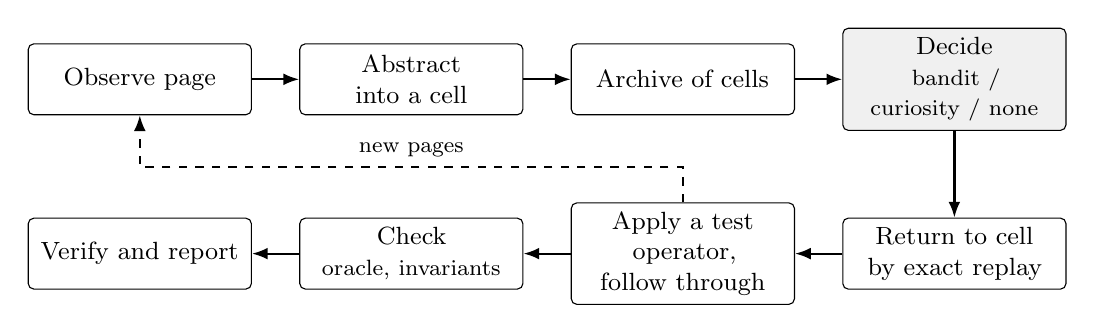
\begin{tikzpicture}[
  box/.style={draw, rounded corners=2pt, align=center, minimum height=0.9cm,
              text width=2.6cm, font=\small, execute at begin node={\hyphenpenalty=10000}},
  arr/.style={-{Latex[length=2mm]}, thick}]
  \node[box] (obs) {Observe page};
  \node[box, right=0.6cm of obs] (abs) {Abstract into a cell};
  \node[box, right=0.6cm of abs] (arc) {Archive of cells};
  \node[box, right=0.6cm of arc, fill=gray!12] (dec) {Decide\\\footnotesize bandit / curiosity / none};
  \node[box, below=1.1cm of dec] (ret) {Return to cell by exact replay};
  \node[box, left=0.6cm of ret] (op) {Apply a test operator, follow through};
  \node[box, left=0.6cm of op] (chk) {Check\\\footnotesize oracle, invariants};
  \node[box, left=0.6cm of chk] (ver) {Verify and report};
  \draw[arr] (obs) -- (abs);
  \draw[arr] (abs) -- (arc);
  \draw[arr] (arc) -- (dec);
  \draw[arr] (dec) -- (ret);
  \draw[arr] (ret) -- (op);
  \draw[arr] (op) -- (chk);
  \draw[arr] (chk) -- (ver);
  \draw[arr, dashed] (op.north) -- ++(0,0.45) -| node[pos=0.25, above, font=\footnotesize]{new pages} (obs.south);
\end{tikzpicture}
\caption{The hybrid tester's loop. Every replayed action counts towards the budget.}
\label{fig:hybrid}
\end{figure}

\section{Page abstraction}
\label{sec:abstraction}

Each page becomes a small symbolic \emph{cell}, computed deterministically from the markup:

\begin{itemize}[noitemsep]
  \item the page kind, from a closed vocabulary (home, list, detail, form, review, outcome,
        info, login, error, other);
  \item the URL path with identifiers replaced (\code{/orders/\{n\}});
  \item the main heading;
  \item whether the form on the page is empty, partly filled or full;
  \item whether an error or alert is shown;
  \item whether the page offers a submit action.
\end{itemize}

Controls get roles from markup cues: submit, edit, remove, add, back, navigate. Two rules
came from development evidence. Links and buttons in the page's navigation, header or
footer are never "submit": they start a new journey rather than complete the current one.
And role cues match word prefixes, so "Saving" and "Save" share a role.

Experiment 2 showed that the network does not learn these distinctions by itself, and the
literature finds that the choice of state abstraction drives results in both web
testing~\cite{chang2023webqt, liu2026webgui} and count-based
exploration~\cite{tang2017exploration}. The granularity was tuned on development
applications only: exact field combinations gave 150--225 cells on one application, so form
state was reduced to empty, partial and full, which gave about 20.

\section{Archive with exact return}
\label{sec:archive}

The tester keeps an archive of every cell it has reached, with the shortest known action
sequence to it, its visit count, and the operators already tried there. At the start of an
excursion it chooses a cell with probability proportional to a weight
\begin{equation}
  w(c) = \frac{1}{\sqrt{1 + n_c}}\cdot\Big(1 + \frac{\min(u_c, 10)}{5}\Big)\cdot
         \frac{1}{1 + 2 f_c}\cdot \rho_c \cdot \Big(1 + \beta_d\,\frac{\min(d_c, 30)}{30}\Big),
\end{equation}
where $n_c$ is the number of visits, $u_c$ the number of untried operators, $f_c$ the
number of failed returns, $\rho_c$ is 1 if enough of the episode remains after reaching the
cell and 0.1 otherwise, $d_c$ the cell's depth, and $\beta_d = 2$ a preference for depth
(faults sit many steps into a workflow). The tester then \emph{returns} to the cell by
replaying its path exactly, and acts from there. This is
Go-Explore~\cite{ecoffet2021first}: poor exploration comes from forgetting how to get back to
promising states, and the deep, unfound faults of Experiment 1 were exactly that case.

Paths are pruned of steps that change neither the page nor the cell, and every replayed
action counts towards the interaction budget, so returning is not a hidden advantage. One
replay bug, in which pruning removed steps that raised a notice the next step depended on,
was found on a development application and fixed; failed returns fell from 6 of 14 to 0 of
28.

\section{Test operators}
\label{sec:operators}

From a cell the tester applies a \emph{test operator}, a short procedure from standard test
design~\cite{myers2011art, beizer1990software}:

\begin{itemize}[noitemsep]
  \item \code{complete\_step}: fill the form validly and submit (the path deeper);
  \item \code{choose\_option}: take each option of a dropdown in turn (equivalence classes);
  \item \code{invalid\_input}: enter an empty value, a value of the wrong type, or a boundary
        minimum or maximum (boundary-value analysis);
  \item \code{edit\_after\_review}: reach a review step, go back and change an earlier
        answer (state-transition testing);
  \item \code{back\_and\_resume}, \code{reload\_and\_resume}: interrupt a flow and continue;
  \item \code{double\_submit}: submit twice in quick succession;
  \item \code{collection\_churn}: add and remove items in a collection;
  \item \code{combine} (development option, not adopted): two deviations on one form, such
        as a dropdown option together with an invalid field (pairwise testing);
  \item \code{browse\_list} (option, Section~\ref{sec:v3-options}): sort or filter a list,
        page forward, and open an item on a later page.
\end{itemize}

Each operator then \emph{follows through}: it continues the task to submission, for up to
four submissions, because a deviation usually shows its effect only on a later page. When a
page offers several submit actions (for example, "Update bag" and "Go to checkout"),
operators take them in turn on repeat visits. Operators are chosen by technique, not from
any application's faults. They are how the tester leaves the happy path, which the LLM
progress reward could not do.

\section{The decision layer}
\label{sec:decision}

The decision layer chooses which cell to return to and which operator to apply on which
target. Three variants exist; each is an arm.

\paragraph{No learner (\code{hybrid\_nolearn}).} Cells by the archive weight; at a cell,
untried (operator, target) pairs first, in random order. This is the non-learning
reference.

\paragraph{Thompson-sampling bandit (\code{hybrid\_bandit}).} A Bayesian bandit learns,
online inside the application, which operator pays off on which kind of target. Its keys
are semantic and back off from specific to general:
\[
  (\text{page kind}, \text{operator}, \text{target type}) \;\rightarrow\;
  (\text{operator}, \text{target type}) \;\rightarrow\; (\text{operator}).
\]
Each key has a $\mathrm{Beta}(\alpha, \beta)$ posterior over the probability that the
operator produces an interesting outcome. A specific key's prior is the more general keys'
evidence, discounted by 0.3, so a new combination starts from what similar ones did. At each
decision the tester samples from every candidate's posterior and takes the best
sample~\cite{thompson1933likelihood, russo2018tutorial}. The reward is the tester's own
observation, never the seeded-fault oracle: an alert shown, new cells reached, or an
invariant candidate. A bandit was chosen over a deep network for three reasons:
Experiment 1 found no gain from bootstrapped multi-step learning; a 2{,}000-interaction run
makes only about 50--135 decisions, enough for a bandit over a few dozen interpretable keys
but far too few for a network; and keys based on page kinds, not application text, can carry
across applications.

\paragraph{Curiosity Q-learning (\code{hybrid\_curiosity}).} This variant adopts the
literature's design for the free exploration steps between operators. Following
WebExplor~\cite{zheng2021webexplor} and WebRLED~\cite{gu2025webrled}, a tabular
Q-learner over cells is rewarded on every step for curiosity:
\begin{equation}
  r = \frac{1}{\sqrt{N(c, a, c')}} + 0.5\cdot\mathbb{1}[c' \text{ not yet seen this episode}],
\end{equation}
where $N(c, a, c')$ counts the transition. It learns with $\alpha = 0.5$, $\gamma = 0.9$ and
$\epsilon = 0.1$, with untried actions initialised optimistically at
$R_{\max}/(1-\gamma)$, so that an action that changes nothing cannot outrank untried ones by
bootstrapping off itself. Being off-policy, it learns from every transition, about 2{,}000
updates per run, against about 135 outcomes for the bandit. A standalone tester built only
from these components (no operators, no bandit) was also run, as
\code{dev\_curiosity\_rl}.

\section{Options for the final tuning round}
\label{sec:v3-options}

After the held-out evaluation (Chapter~\ref{chap.7}) and the rebuild of the development
applications, three options were added, each switched on in its own tuning arm:

\begin{itemize}
  \item \textbf{\code{browse\_list}} (\code{dev\_v3\_browse}). The held-out evaluation
        exposed a blind spot: the operators work on forms, and no operator pages through a
        list. This operator applies a sort or filter control, presses "next" or "load more"
        up to twice, and opens an item on the later page.
  \item \textbf{Custom clickables} (\code{dev\_v3\_clickables}). The registry also offers
        elements made clickable by ARIA roles, click handlers or styling, such as kanban
        cards and tab strips.
  \item \textbf{Failure feedback} (\code{dev\_v3\_failfeedback}). Cells where a browser
        error followed an action get extra archive weight (up to $\times 3$), since code
        that already misbehaves is likelier to misbehave again nearby.
\end{itemize}

The curiosity variant (\code{dev\_v3\_curiosity}) is the fourth tuning arm.

\section{Development rounds}
\label{sec:devrounds}

The design was tuned on development data only: the six benchmark applications, a generated
application family, Gitea, and the eight development suite applications
(Chapter~\ref{chap.6}). Each round compared arms on the same applications and seeds, and
ended with a recorded decision. Table~\ref{tab:devrounds} lists them.

\begin{table}[H]
\centering
\small
\caption{Development rounds of the hybrid tester and their decisions.}
\label{tab:devrounds}
\begin{tabularx}{\textwidth}{@{}lX X@{}}
\toprule
Round & Tested & Decision \\
\midrule
Benchmark 1 & bandit, no learner, random (4 apps) & discarded (code changed mid-round); replay bug found and fixed \\
Benchmark 2 & bandit vs no learner, with clean builds (6 apps) & validation invariant narrowed; form fixes \\
Benchmark 3 & free-exploration variants & depth preference and weighted exploration adopted \\
Benchmark 4--5 & which submit actions a cell records & cells record \emph{whether} a submit is offered \\
Benchmark 6--7 & whole-word vs prefix matching of role cues & prefix matching adopted \\
Suite 1 & bandit vs no learner, 8 suite apps & site navigation never submits; submit actions taken in turn \\
Suite 2 & the same after the fix, 14 apps & kept; learner not ahead \\
Suite 3 & two corrected bandit rewards (novelty, surprise) & no difference: reward not the bottleneck \\
Suite 4 & pairwise operator + technique-first choice & worse; not adopted \\
Suite 5 & curiosity Q-learning, in the hybrid and standalone & neither adopted \\
\bottomrule
\end{tabularx}
\end{table}

\begin{table}[H]
\centering
\small
\caption{All arms on the same runs: suite rounds 2--5, 14 applications $\times$ 3 seeds.
Difference is the per-application mean $T$ against \code{hybrid\_nolearn}, with a bootstrap
interval over applications (negative = faster).}
\label{tab:devarms}
\begin{tabular}{@{}lrrrl@{}}
\toprule
Arm & Found a fault & Median $T$ & Mean $T$ & Difference [95\% interval] \\
\midrule
\code{hybrid\_nolearn} & 32 / 42 & 742 & 889 & reference \\
\code{hybrid\_bandit} & 30 / 42 & 335 & 840 & $-49$ $[-279, +190]$ \\
\code{dev\_bandit\_surprise} & 31 / 42 & 586 & 844 & $-46$ $[-257, +143]$ \\
\code{dev\_bandit\_novelty} & 31 / 42 & 486 & 854 & $-35$ $[-252, +190]$ \\
\code{dev\_pairwise\_bandit} & 27 / 42 & 757 & 943 & $+53$ $[-121, +227]$ \\
\code{dev\_hybrid\_curiosity} & 29 / 42 & 612 & 978 & $+89$ $[-38, +202]$ \\
\code{dev\_pairwise\_nolearn} & 26 / 40 & 1{,}069 & 1{,}046 & $+119$ $[-37, +281]$ \\
\code{dev\_curiosity\_rl} & 17 / 42 & 2{,}000 & 1{,}313 & $+423$ $[+142, +744]$ \\
\code{random} & 18 / 42 & 2{,}000 & 1{,}355 & $+465$ $[+178, +790]$ \\
\bottomrule
\end{tabular}
\end{table}

\paragraph{Is the learner helping?} The top four arms in Table~\ref{tab:devarms} are
statistically tied. \code{hybrid\_nolearn} verified a fault in the most runs, and
\code{hybrid\_bandit} was fastest when it found one. No learner variant improved on no
learner: three bandit reward signals, the pairwise operator, and curiosity Q-learning. The
standalone curiosity tester was fast on shallow faults but never found the deep ones, and
was significantly worse than the hybrid, level with random. It is a tester built from the
published components, not a reproduction of WebExplor or WebRLED; their published results
(coverage and crash-type failures over long runs) are not contradicted by it.

The design leaves the learner little to decide, for four reasons. On about 5 of the 14
applications a fault is found within the first few decisions, before learning can matter.
The faults no arm finds need two deviations in one walk (for example, express delivery
\emph{and} an empty address), which choosing one operator more cleverly cannot produce. The
option space is small: about 28 cells times 8 operators can mostly be covered in about 135
decisions, so trying untried options systematically already does most of the work. And
operators with many targets crowd out the rest: invalid input took 30\% of all decisions
because pages have many fields. This agrees with the Humanoid authors' observation that
their learned model was not the main reason for their gains~\cite{li2019humanoid}: on
functional faults, the structure (abstraction, archive with exact return, operators) does
the work.

\chapter{Test Applications and Evaluation Methodology}
\label{chap.6}

A tester can only be evaluated on applications whose faults are known. This chapter
describes the four sets of test applications (Sections~\ref{sec:benchmark}--\ref{sec:external}),
how an application is admitted before any agent touches it
(Section~\ref{sec:admission}), how applications were split between development and
evaluation (Section~\ref{sec:split}), and the metrics and statistics
(Section~\ref{sec:stats}). Section~\ref{sec:threats} states the threats to validity.

\section{The six-application benchmark}
\label{sec:benchmark}

Six small web applications were built to one design contract for the v1 experiments: an
account hub, an admin records system, a booking desk, a media library, a shop catalogue and a
support portal. Each carries two seeded faults, 12 in total, in five classes: calculation
error, constraint bypass, persistence failure, state corruption and broken transition. Some
faults sit 9--16 contextual steps deep. Two applications (the shop catalogue and the
booking desk) were used during development; the other four stayed pristine until the
transfer experiment.

\section{The generated application family}

For Experiment 2, a seeded generator produced twelve variants of one loan-request workflow.
They differ in vocabulary, structure and decoys, and each was admitted by the same validator
as the benchmark (Section~\ref{sec:exp2}).

\section{The development suite}
\label{sec:devsuite}

Eight applications were built to be genuinely different from each other and from the
benchmark: different domains, architectures and stacks (Table~\ref{tab:devsuite}). They were
first built as zero-dependency applications. Then, at the project owner's request, they were
rebuilt as full-stack applications. Each now has its own database (PostgreSQL or MongoDB), a
sign-in page and a richer data model. The five rebuilt last were also enlarged to at least 12
views, 3 entities with full create, read, update and delete, 5 interaction patterns, and 2
new faults that are not about forms.

\begin{table}[H]
\centering
\small
\caption{The development suite (version 2).}
\label{tab:devsuite}
\begin{tabularx}{\textwidth}{@{}l X l l r r@{}}
\toprule
App & Domain and architecture & Server & Database & Faults & Crash \\
\midrule
tidewater & personal banking; single-page app over a JSON API & Python & PostgreSQL & 3 & -- \\
clinicflow & clinic front desk; server-rendered branching wizard & Python & PostgreSQL & 5 & -- \\
stackroom & stockroom inventory; data grid with server-side paging, sorting, bulk actions & Python & PostgreSQL & 5 & 2 \\
ledgerly & expense claims with multi-role approval; server-rendered forms & Node.js & PostgreSQL & 5 & -- \\
bagstreet & small shop; server-rendered pages and HTML forms & Python & MongoDB & 5 & -- \\
helpline & broadband care desk; pages with HTML fragment updates & Python & MongoDB & 7 & 2 \\
orbit & kanban boards; modal-heavy single-page app & Node.js & MongoDB & 5 & 2 \\
wayfarer & trip itinerary builder; client drafts and sealed server versions & Node.js & MongoDB & 6 & 2 \\
\midrule
& & & & 41 & 8 \\
\bottomrule
\end{tabularx}
\end{table}

\paragraph{Isolation between sessions.} Every signed-in browser context gets its own data
partition: a schema per session in PostgreSQL, a database per session in MongoDB. This
resets the application between episodes and keeps parallel runs independent. The database
drivers are vendored and pinned, so a build needs no network.

\paragraph{Crash-type faults.} Four applications also carry two crash-type faults each
(Section~\ref{sec:crash}), so that the tuned tester is exercised on the kind of failure the
external benchmark counts. By the project owner's decision only a subset of applications has
them. Orbit's were admitted (40 of 40 checks, including Docker); helpline, stackroom and wayfarer were
admitted with all checks passing (44, 40 and 41 checks, including Docker).

\section{The validation suite}
\label{sec:valsuite}

Eight further applications were planned by an independent agent working only from the
suite's design contract, without access to the tester's code or results, and built for the
held-out evaluation (Table~\ref{tab:valsuite}). Each has three seeded faults, 24 in total,
and each was admitted with 20 of 20 checks. They were evaluated in their first version
(without a database server or sign-in) and have not been changed since.

\begin{table}[H]
\centering
\small
\caption{The validation suite, used once, for the held-out evaluation.}
\label{tab:valsuite}
\begin{tabularx}{\textwidth}{@{}l X l r@{}}
\toprule
App & Domain & Stack & Faults \\
\midrule
dutyday & a food bank's volunteer rota & Python, SQLite & 3 \\
fosterly & an application to become a foster carer, saved section by section & Node.js, JSON files & 3 \\
larder & a personal recipe box with scaling and unit conversion & Node.js, JSON files & 3 \\
markbook & a teacher's markbook with a student view & Python, SQLite & 3 \\
quizcraft & a survey editor with undo, redo and a respondent preview & Python, SQLite & 3 \\
sideline & a football league's results, confirmations and table & Python, SQLite & 3 \\
skylark & a nature group's bird-sightings register with a paged feed & Node.js, JSON files & 3 \\
tally & a club election by ranked ballot & Node.js, JSON files & 3 \\
\bottomrule
\end{tabularx}
\end{table}

\section{The external benchmark}
\label{sec:external}

To compare with published RL web testers on their own ground, the final evaluation uses the
six subject applications of WebExplor~\cite{zheng2021webexplor}, which WebRLED's first
benchmark~\cite{gu2025webrled} also uses:
\begin{itemize}[noitemsep]
  \item Dimeshift, an expense tracker;
  \item Pagekit, a content management system, tested in its admin area;
  \item Splittypie, which splits bills;
  \item Phoenix, a Trello clone;
  \item Retroboard, a retrospective board;
  \item Petclinic, the Spring demonstration application.
\end{itemize}
They are open-source applications not written by this project. They run from the Docker
images of the DIG replication material~\cite{biagiola2019diversity}, which instrument the
client JavaScript with Istanbul, so branch coverage is measured the way the papers measured
it. To keep the comparison honest, nobody looked at these applications before the re-tuned
tester was frozen and the comparison pre-registered (Section~\ref{sec:extresults}).

\section{Admission}
\label{sec:admission}

Before any agent runs on an application, a harness must admit it mechanically. For each
fault, a scripted \emph{witness} trace must trigger the fault's assertion on the faulty build
and not on that fault's control build. The witness must replay deterministically and
minimise to a short reproduction. Benign traces must trigger nothing. A random walk on the
clean build must produce no candidate. The faulty build must differ from the clean build
\emph{only} by the declared patches; a diff audit checks this. The development suite adds a
data-model contract (seeded record counts per entity), a breadth contract (views, entities,
interaction patterns), sign-in checks, crash checks and a Docker build. An application that
fails any check is not used. A diversity check also confirms that the suite's applications
do not share code (the largest overlap was 3.2\%).

\section{Data split and independence}
\label{sec:split}

\begin{itemize}
  \item \textbf{Development} (used for tuning and design decisions): the six benchmark
        applications, the generated family, Gitea (a real open-source application, as a
        non-admin user), and the eight development suite applications.
  \item \textbf{Held-out}: the eight validation applications, used once, by the
        pre-registered evaluation of Chapter~\ref{chap.7}.
  \item \textbf{External}: the WebExplor and WebRLED subject applications, used once, by
        the final comparison.
\end{itemize}

The split was fixed before any agent ran on the suites. Development results are tuning data.
They are never presented as evidence of generalisation, and the held-out result belongs to
the version of the tester frozen before it ran.

\section{Metrics and statistics}
\label{sec:stats}

\paragraph{Outcome.} For a run with budget $B$, $T$ is the number of interactions until the
first verified fault. Every browser action counts, including replays and returns. A run that
finds nothing is right-censored at $T = B$.

\paragraph{Per arm.} The \emph{discovery rate} is the share of runs that verified at least
one fault. The \emph{restricted mean} of $T$ (RMST) averages $T$
over runs with censored runs at $B$. \emph{Distinct faults} counts how many of the seeded
faults an arm verified in at least one run. Clean-build control runs give the false-positive
count. For the tuning round two descriptive metrics were added. \emph{Unique failures} counts
distinct browser-error signatures (console, page and failed-request errors). \emph{JavaScript
coverage} is the share of the application's client-side code executed, measured with V8's
precise coverage through the Chrome DevTools Protocol, attached before the first navigation.

\paragraph{Comparisons.} Applications differ far more than seeds do, so the
\emph{application} is the unit of inference. For two arms, the per-application difference
in restricted mean $T$ is computed on matched (application, seed) pairs; the median across
applications summarises it, with a 95\% bootstrap interval resampling
applications. The stratified log-rank test is
secondary. The pre-registered decision rule:
\begin{itemize}[noitemsep]
  \item \emph{supported} if the median difference is negative (faster) and its interval
        excludes zero;
  \item \emph{refuted} if it is positive and the interval excludes zero;
  \item otherwise \emph{inconclusive}.
\end{itemize}

\paragraph{Pre-registration.} For every pre-registered experiment, the hypotheses, arms,
applications, budget, seeds, analysis code and decision rule were committed to the
repository, and the commit was tagged before any agent ran on the evaluation
applications~\cite{klees2018evaluating}. Deviations, such as rerunning a job lost to an
infrastructure failure, follow rules written in advance and are reported.

\section{Threats to validity}
\label{sec:threats}

\begin{itemize}
  \item \textbf{Same developer.} The test applications and their seeded faults were built
        by the same project as the tester. Independent planning of the validation suite and
        the external benchmark reduce, but do not remove, this threat.
  \item \textbf{Seeded faults.} Seeded faults are an incomplete proxy for real
        faults, and the oracle sees only what was seeded.
  \item \textbf{Scale.} Eight applications per evaluation leave wide intervals at the
        application level. Small effects cannot be told apart from noise.
  \item \textbf{Fault difficulty.} If the held-out faults are shallow, every arm finds them
        and differences compress. Chapter~\ref{chap.7} reports that this happened.
  \item \textbf{Tuning leakage.} Decisions made on development data can overfit it; the
        held-out and external evaluations exist to measure that.
\end{itemize}

\chapter{Evaluation}
\label{chap.7}

This chapter reports three evaluations of the hybrid tester. The pre-registered held-out
evaluation on the validation suite (Section~\ref{sec:heldout}) is complete. The final tuning
round on the rebuilt development suite (Section~\ref{sec:tuning}) and the external comparison
with WebExplor and WebRLED (Section~\ref{sec:extresults}) follow it.

\section{Held-out evaluation (pre-registered)}
\label{sec:heldout}

\subsection{Design}

The pre-registration was frozen on the project owner's approval, and the commit was tagged,
before any agent ran on any validation application.

\begin{itemize}
  \item \textbf{Applications}: the eight validation applications (Table~\ref{tab:valsuite}),
        24 seeded faults.
  \item \textbf{Arms}:
        \begin{itemize}[noitemsep]
          \item \code{random}, uniform over the page's valid actions;
          \item \code{hybrid\_nolearn}, the primary arm;
          \item \code{hybrid\_bandit};
          \item \code{v1\_dqn\_pretrained}, v1's best AC-DQN arm from Experiment 1: pretrained
                without the LLM reward and adapting online, using that experiment's own
                checkpoints. Seed $s$ loads the checkpoint of fold $s \bmod 6$, pretraining
                seed $s \bmod 3$.
        \end{itemize}
  \item \textbf{Runs}: seeds 0--4, $B = 2{,}000$ interactions, 160 hunts, plus 32 clean-build
        control runs (one per arm and application). The run took about seven and a half
        hours with four workers and no other workload.
  \item \textbf{Hypotheses} (difference in restricted mean $T$, decision rule of
        Section~\ref{sec:stats}):
        \begin{itemize}[noitemsep]
          \item H1 (primary): the hybrid tester is faster than random;
          \item H2: the bandit makes the hybrid faster;
          \item H3: the hybrid with the bandit is faster than random;
          \item H4: the hybrid is faster than v1's best AC-DQN.
        \end{itemize}
\end{itemize}

One of 192 jobs failed for an infrastructure reason: Windows held a file lock while the
temporary build folder of a clean-build control was being deleted. As pre-registered, the job
was rerun unchanged; it completed with no finding.

\subsection{Results}

\begin{table}[H]
\centering
\small
\caption{Held-out evaluation: pre-registered comparisons (negative $\Delta$ = first arm faster).}
\label{tab:heldout-h}
\resizebox{\textwidth}{!}{%
\begin{tabular}{@{}llrrrrl@{}}
\toprule
& Comparison & Median $\Delta$ & 95\% interval & Apps favouring & Log-rank $p$ & Verdict \\
\midrule
H1 & \code{hybrid\_nolearn} $-$ \code{random} & $-324$ & $[-665, +148]$ & 6/8 & 0.159 & inconclusive \\
H2 & \code{hybrid\_bandit} $-$ \code{hybrid\_nolearn} & $+86$ & $[-304, +285]$ & 4/8 & 0.781 & inconclusive \\
H3 & \code{hybrid\_bandit} $-$ \code{random} & $-191$ & $[-801, +67]$ & 5/8 & 0.180 & inconclusive \\
H4 & \code{hybrid\_nolearn} $-$ \code{v1\_dqn\_pretrained} & $+42$ & $[-196, +574]$ & 4/8 & 0.276 & inconclusive \\
\bottomrule
\end{tabular}}
\end{table}

\begin{table}[H]
\centering
\small
\caption{Held-out evaluation per arm (40 runs each).}
\label{tab:heldout-arms}
\resizebox{\textwidth}{!}{%
\begin{tabular}{@{}lrrrrr@{}}
\toprule
Arm & Found a fault & RMST & Faults per run & Distinct faults & Clean false positives \\
\midrule
\code{v1\_dqn\_pretrained} & 34 (0.85) & \textbf{595} & 1.18 & 17 / 24 & 0 / 8 \\
\code{hybrid\_nolearn} & 30 (0.75) & 737 & 1.15 & 18 / 24 & 0 / 8 \\
\code{hybrid\_bandit} & 34 (0.85) & 769 & \textbf{1.23} & \textbf{19} / 24 & 0 / 8 \\
\code{random} & 32 (0.80) & 978 & 1.00 & 13 / 24 & 0 / 8 \\
\bottomrule
\end{tabular}}
\end{table}

\begin{table}[H]
\centering
\small
\caption{Held-out evaluation per application: runs that found a fault (of 5) and mean $T$.}
\label{tab:heldout-apps}
\begin{tabular}{@{}lllll@{}}
\toprule
App & \code{random} & \code{v1\_dqn\_pretrained} & \code{hybrid\_nolearn} & \code{hybrid\_bandit} \\
\midrule
dutyday & 4/5 $\cdot$ 1{,}217 & \textbf{5/5 $\cdot$ 281} & 4/5 $\cdot$ 788 & 4/5 $\cdot$ 778 \\
fosterly & 5/5 $\cdot$ 1{,}262 & 4/5 $\cdot$ 763 & 4/5 $\cdot$ 681 & \textbf{5/5 $\cdot$ 370} \\
larder & 5/5 $\cdot$ 411 & 5/5 $\cdot$ 407 & \textbf{5/5 $\cdot$ 211} & 5/5 $\cdot$ 393 \\
markbook & 1/5 $\cdot$ 1{,}805 & \textbf{4/5 $\cdot$ 567} & 3/5 $\cdot$ 1{,}141 & 4/5 $\cdot$ 1{,}442 \\
quizcraft & 5/5 $\cdot$ 299 & 5/5 $\cdot$ 97 & \textbf{5/5 $\cdot$ 81} & 5/5 $\cdot$ 366 \\
sideline & 2/5 $\cdot$ 1{,}623 & 1/5 $\cdot$ 1{,}759 & \textbf{4/5 $\cdot$ 620} & 3/5 $\cdot$ 822 \\
skylark & 5/5 $\cdot$ 980 & \textbf{5/5 $\cdot$ 614} & 0/5 $\cdot$ 2{,}000 & 3/5 $\cdot$ 1{,}696 \\
tally & 5/5 $\cdot$ \textbf{229} & 5/5 $\cdot$ 276 & 5/5 $\cdot$ 376 & 5/5 $\cdot$ 284 \\
\bottomrule
\end{tabular}
\end{table}

All four pre-registered comparisons are inconclusive (Table~\ref{tab:heldout-h}). As the
pre-registration anticipated, eight applications give the median rule wide intervals, and no
comparison was supported or refuted. The per-fault counts are in
Appendix~\ref{app:faults}.

\subsection{What the held-out data shows (descriptive)}

\begin{enumerate}
  \item \textbf{The held-out faults were easier for random exploration than the development
        ones.} Random verified a fault in 80\% of runs, against 43\% (18 of 42) on the
        development suite. Several faults sit one or two interactions from a page that
        random visits constantly. Three faults were verified in 5 of 5 runs by every arm,
        which compresses every difference.
  \item \textbf{The hybrid arms reached the deeper faults.} 22 of the 24 faults were
        verified by at least one arm; two by none. Of the 16 faults random verified in at
        most one of five runs, the two hybrid arms together verified 14 at least once, and
        \code{v1\_dqn\_pretrained} 9. Nine faults were verified by a hybrid arm and by no
        random run. This is where test operators help: completing forms validly, invalid
        input, edits after review.
  \item \textbf{One clear blind spot: list paging.} All three skylark faults sit behind its
        feed's "Load more" button. Random presses it often by chance. The hybrid's operators
        work on forms and none pages through a list, so \code{hybrid\_nolearn} reached the
        right pages in every run but never repeated the paging (0 of 5). This cost H1 one
        of its eight applications. It was reported, not fixed, because the code was frozen;
        it motivated the \code{browse\_list} operator (Section~\ref{sec:v3-options}).
  \item \textbf{v1's pretrained AC-DQN did better here than on its own benchmark}: discovery
        0.85 and the lowest mean time, notably on dutyday and markbook. Whether that
        reflects the method or the applications' shallower faults cannot be separated with
        eight applications (H4 inconclusive).
  \item \textbf{The learner (H2).} \code{hybrid\_bandit} found a fault in more runs than
        \code{hybrid\_nolearn} (34 against 30) and more distinct faults (19 against 18), with
        a slightly higher mean time (769 against 737). As in development, the learner is
        not distinguishable from no learner.
  \item \textbf{Zero false positives.} No clean-build control verified a seeded fault
        (0 of 32 runs).
\end{enumerate}

\paragraph{Specification-free invariants.} As pre-registered, they are reported separately.
They flagged no seeded fault for any arm. On clean builds they produced three reproduced
candidates (two for \code{hybrid\_nolearn}, one for \code{hybrid\_bandit}), all on
quizcraft's editor, all of the form "an entered value is gone after reload". On inspection,
quizcraft keeps its working copy in page memory until the user saves, so losing unsaved
edits on reload is intended. They are false alarms: the reload invariant cannot tell saved
state from unsaved state.

\section{Tuning round v3 on the rebuilt development suite}
\label{sec:tuning}

\subsection{Design}

After the held-out evaluation, the development suite was rebuilt (Section~\ref{sec:devsuite})
and the tester re-tuned on it before the external comparison. Eight arms ran on the eight
development applications with seeds 0--2, 192 runs of 2{,}000 interactions:

\begin{itemize}[noitemsep]
  \item the references: \code{random}, \code{hybrid\_nolearn}, \code{hybrid\_bandit} and
        \code{v1\_dqn\_pretrained};
  \item one option each (Section~\ref{sec:v3-options}):
        \begin{itemize}[noitemsep]
          \item \code{dev\_v3\_browse},
          \item \code{dev\_v3\_clickables},
          \item \code{dev\_v3\_curiosity},
          \item \code{dev\_v3\_failfeedback}.
        \end{itemize}
\end{itemize}

Each run records verified faults (including crash-type faults), unique failures and
JavaScript coverage. These are development data: they choose the configuration to freeze,
and are not evidence of generalisation.

\subsection{Results}

All 192 runs completed, none failed. Table~\ref{tab:tuning-arms} summarises each arm.
Table~\ref{tab:tuning-matched} compares each arm with \code{hybrid\_nolearn} on matched
(application, seed) pairs.

\begin{table}[H]
\centering
\small
\caption{Tuning round v3 per arm: 24 runs each on the eight rebuilt development
applications, which hold 41 seeded faults (8 of them crash-type).}
\label{tab:tuning-arms}
\resizebox{\textwidth}{!}{%
\begin{tabular}{@{}lrrrrrr@{}}
\toprule
Arm & Found a fault & RMST & Distinct faults & Crash faults & Unique failures / run & JS coverage \\
\midrule
\code{dev\_v3\_failfeedback} & 21 / 24 & \textbf{450} & 19 / 41 & 3 / 8 & 3.79 & 0.893 \\
\code{random} & \textbf{23} / 24 & 498 & 19 / 41 & 1 / 8 & 5.38 & 0.861 \\
\code{dev\_v3\_browse} & 20 / 24 & 545 & 19 / 41 & 3 / 8 & 3.12 & 0.885 \\
\code{hybrid\_nolearn} & 21 / 24 & 560 & 19 / 41 & \textbf{4} / 8 & 2.88 & 0.896 \\
\code{v1\_dqn\_pretrained} & 20 / 24 & 564 & 19 / 41 & 2 / 8 & 4.75 & \textbf{0.909} \\
\code{dev\_v3\_clickables} & 19 / 24 & 638 & 17 / 41 & 3 / 8 & 2.50 & 0.891 \\
\code{dev\_v3\_curiosity} & 20 / 24 & 650 & 16 / 41 & 2 / 8 & \textbf{5.67} & 0.894 \\
\code{hybrid\_bandit} & 19 / 24 & 692 & 16 / 41 & 3 / 8 & 2.83 & 0.896 \\
\bottomrule
\end{tabular}}
\end{table}

\begin{table}[H]
\centering
\small
\caption{Tuning round v3 against \code{hybrid\_nolearn}: per-application mean difference in
$T$ (negative = faster), median over applications with a 95\% bootstrap interval. Apps
with no difference are not counted as faster or slower.}
\label{tab:tuning-matched}
\begin{tabular}{@{}lrrc@{}}
\toprule
Arm & Median & 95\% interval & Apps faster / slower \\
\midrule
\code{dev\_v3\_browse} & $-20$ & $[-79, 0]$ & 6 / 1 \\
\code{dev\_v3\_failfeedback} & 0 & $[-379, 0]$ & 3 / 1 \\
\code{random} & $-18$ & $[-285, +186]$ & 5 / 3 \\
\code{v1\_dqn\_pretrained} & $-45$ & $[-182, +265]$ & 5 / 3 \\
\code{dev\_v3\_clickables} & 0 & $[0, +286]$ & 0 / 3 \\
\code{dev\_v3\_curiosity} & $+43$ & $[-248, +549]$ & 4 / 4 \\
\code{hybrid\_bandit} & $+140$ & $[+112, +416]$ & 1 / 7 \\
\bottomrule
\end{tabular}
\end{table}

\paragraph{Reading.}
\begin{itemize}
  \item \textbf{\code{browse\_list} helps consistently but modestly.} It was faster on six of
        seven applications and slower on one, and lost no fault.
  \item \textbf{Failure feedback gave the best restricted mean time} (450).
  \item \textbf{Custom clickables did not help.} They were never faster, and verified fewer
        distinct faults.
  \item \textbf{The bandit was slower than no learner} on seven of eight applications. Its
        interval excludes zero.
  \item \textbf{Curiosity Q-learning triggered the most unique browser errors} (5.67 per
        run) but verified fewer seeded faults.
  \item \textbf{Random exploration was strong on these applications.} It found a fault in 23
        of 24 runs and triggered many errors, but verified only one crash-type fault.
  \item \textbf{The rebuilt applications are hard.} 15 of the 41 faults were verified by no
        arm.
\end{itemize}

\subsection{Configuration chosen}

The two options that did not hurt any measure, \code{browse\_list} and failure feedback,
were combined (\code{dev\_v3\_combined}) and checked in 24 further runs on the same
applications and seeds before freezing. The combination found a fault in 22 of 24 runs,
with restricted mean $T$ 465. It verified 22 of the 41 faults, more than any single arm, and
4 of the 8 crash-type faults. Against \code{hybrid\_nolearn} it was faster on six of seven
applications (median $-52$, interval $[-145, 0]$). It was frozen as \code{hybrid\_final},
and the commit was tagged before anyone looked at the external benchmark's applications.
Custom clickables and the bandit were not adopted.

\section{Comparison with WebExplor and WebRLED}
\label{sec:extresults}

\subsection{Design}

The WebRLED paper~\cite{gu2025webrled} reports results on WebExplor's six subject
applications (Dimeshift, Pagekit, Splittypie, Phoenix, Retroboard and Petclinic), with
one-hour runs and five repetitions. WebExplor averaged 55.54\% client-side branch coverage
and 3.1 failures; WebRLED averaged 64.18\% and 4.1. Coverage was measured with Istanbul on
the instrumented client code. Failures were console errors, deduplicated by hand.

The comparison was pre-registered when \code{hybrid\_final} was frozen, before anyone
looked at the subject applications.
\begin{itemize}
  \item \textbf{Applications.} The same six applications, from the Docker images of the
        DIG replication material~\cite{biagiola2019diversity}, which WebExplor's benchmark
        reuses. Each image instruments its client JavaScript with Istanbul before the
        application starts.
  \item \textbf{Arms.} \code{hybrid\_final}; the hybrid with curiosity Q-learning, the RL
        arm closest to WebExplor and WebRLED; and random.
  \item \textbf{Runs.} One hour of wall-clock time per run, three repetitions (seeds 0--2),
        and a fresh application instance per run, so $3 \times 6 \times 3 = 54$ runs.
  \item \textbf{Measures.} Branch coverage of the instrumented client code, read from
        Istanbul's counters after every step and unioned over the run; and unique failures,
        meaning console errors, page errors and failed requests, deduplicated automatically
        by kind, page and normalised message.
  \item \textbf{Analysis.} A descriptive comparison with the published averages, with no
        significance test against numbers from other machines and runs, and a per-application
        comparison between our arms.
\end{itemize}

Two decisions were made during set-up and recorded before any run. First, Pagekit and
Phoenix start with a sign-in macro using their documented accounts. Second, requests to a
development live-reload server and to web analytics, which the images' pages make, are
answered with an empty response. Left alone, they would add the same console failure to
every run of every arm. Two differences from the published protocol remain and are
reported: three repetitions instead of five, and automatic instead of manual deduplication
of failures.

\subsection{Results}

\pending{Coverage and failures per application against the published numbers; verified
findings.}

\section{Discussion}
\label{sec:discussion}

\pending{Discussion across all evaluations: what the structure contributes, what learning
contributes, how the tester compares with the literature, and the limits of the evidence.}

\chapter{Conclusion and Scope for Further Research}
\label{chap.8}

\section{Conclusion}

\pending{Written after the tuning round and the external comparison. To cover: the answer to
the problem statement; what v1 showed (no transfer, no contextual learning, LLM components
not generalising); what v2 showed (structure finds deep faults with zero false positives;
learning not distinguishable from no learning); the external comparison; the product.}

\section{Limitations}

\pending{Same-developer applications; seeded faults as a proxy; eight applications per
evaluation; the oracle sees only seeded faults; repository intake requires a Dockerfile.}

\section{Scope for further research}

\pending{For example: operators that combine two deviations in one walk; learning across
applications at a scale the literature suggests (tens of applications); specification-free
oracles that tell saved from unsaved state; LLMs used offline to propose operators or
assertions rather than on the decision path.}

\appendix
\chapter{Agent Configurations}
\label{app:a}

\section{Arms}
\label{app:arms}

\begin{table}[H]
\centering
\small
\caption{Every arm used in the evaluations, by generation.}
\label{tab:arms}
\footnotesize
\begin{tabularx}{\textwidth}{@{}l X@{}}
\toprule
Arm & Configuration \\
\midrule
\multicolumn{2}{@{}l}{\emph{Baselines}} \\
\code{random} & uniform choice among the page's valid actions \\
\code{search\_A0} & fixed hand-weighted action priority; no learning \\
\code{search\_S} & fixed linear score over the action features; no learning \\
\midrule
\multicolumn{2}{@{}l}{\emph{v1: action-conditioned DQN (Chapter~\ref{chap.4})}} \\
\code{dqn\_scratch} & learns on the target only; LLM reward on \\
\code{dqn\_scratch\_nollm} & as above, LLM reward off \\
\code{dqn\_pretrained} & pretrained on the other five applications with the LLM reward; residual head adapts \\
\code{dqn\_pretrained\_nollm} & pretrained without the LLM reward; residual head adapts (\code{v1\_dqn\_pretrained} in v2 evaluations) \\
\code{dqn\_zeroshot} & pretrained network frozen; no adaptation \\
\code{bandit\_scratch}, \code{bandit\_pretrained} & the same network with $\gamma = 0$ \\
\midrule
\multicolumn{2}{@{}l}{\emph{v2: hybrid tester (Chapter~\ref{chap.5}); all with depth preference $\beta_d = 2$}} \\
\code{hybrid\_nolearn} & untried (operator, target) pairs first, at random \\
\code{hybrid\_bandit} & Thompson-sampling bandit over semantic keys \\
\code{dev\_bandit\_novelty}, \code{dev\_bandit\_surprise} & bandit rewarded only for new pages / for unexpected responses \\
\code{dev\_pairwise\_bandit}, \code{dev\_pairwise\_nolearn} & pairwise operator and technique-first choice \\
\code{dev\_hybrid\_curiosity} & curiosity Q-learning chooses the free exploration \\
\code{dev\_curiosity\_rl} & standalone curiosity Q-learning tester (no operators) \\
\code{dev\_v3\_browse} & with the \code{browse\_list} operator \\
\code{dev\_v3\_clickables} & with custom clickables in the action registry \\
\code{dev\_v3\_curiosity} & curiosity Q-learning for free exploration (rebuilt suite) \\
\code{dev\_v3\_failfeedback} & archive weight for cells where errors followed actions \\
\bottomrule
\end{tabularx}
\end{table}

\begin{table}[H]
\centering
\small
\caption{Hyperparameters.}
\label{tab:hyper}
\begin{tabularx}{\textwidth}{@{}l X@{}}
\toprule
Component & Values \\
\midrule
Run & budget 2{,}000 interactions; episodes of at most 40 actions \\
v1 network & state encoder 64, action encoder 96, scorer 128 units; dueling \\
v1 learning & Double DQN, 3-step returns, $\gamma = 0.95$, learning rate $3\times10^{-4}$, batch 64, buffer 30{,}000, target update 200, PER $\alpha = 0.6$, $\beta_0 = 0.4$ \\
v1 exploration & guide probability 0.75; target $\epsilon$ 0.50 $\to$ 0.05 over half the budget; pretraining 1{,}500 steps per application \\
v1 reward & LLM weight $\lambda = 1$ (LLM arms), outcome bonus 3, reveal cap 1.5, clip $\pm 6$ \\
Hybrid archive & weight of Section~\ref{sec:archive}; depth preference $\beta_d = 2$ \\
Bandit & Beta posteriors; back-off weight 0.3 \\
Curiosity Q-learning & $\alpha = 0.5$, $\gamma = 0.9$, $\epsilon = 0.1$, episodic bonus 0.5, optimistic initialisation $R_{\max}/(1-\gamma)$ \\
\bottomrule
\end{tabularx}
\end{table}

\section{Held-out evaluation per fault}
\label{app:faults}

\begin{table}[H]
\centering
\small
\caption{Held-out evaluation: runs (of 5) that verified each fault.}
\label{tab:heldout-faults}
\begin{tabular}{@{}lrrrr@{\hspace{1.5cm}}lrrrr@{}}
\toprule
Fault & R & V1 & HN & HB & Fault & R & V1 & HN & HB \\
\midrule
DUTY-1 & 3 & 3 & 0 & 3 & QUIZ-1 & 5 & 5 & 5 & 5 \\
DUTY-2 & 4 & 3 & 4 & 4 & QUIZ-2 & 0 & 2 & 1 & 2 \\
DUTY-3 & 0 & 1 & 1 & 0 & QUIZ-3 & 0 & 1 & 2 & 0 \\
FOST-1 & 5 & 3 & 4 & 5 & SIDE-1 & 0 & 0 & 1 & 1 \\
FOST-2 & 0 & 0 & 0 & 0 & SIDE-2 & 1 & 1 & 2 & 2 \\
FOST-3 & 0 & 2 & 1 & 1 & SIDE-3 & 1 & 0 & 4 & 3 \\
LARD-1 & 1 & 0 & 3 & 4 & SKY-1 & 0 & 3 & 0 & 1 \\
LARD-2 & 5 & 5 & 5 & 5 & SKY-2 & 3 & 1 & 0 & 1 \\
LARD-3 & 1 & 0 & 2 & 1 & SKY-3 & 5 & 5 & 0 & 2 \\
MARK-1 & 0 & 0 & 2 & 2 & TALLY-1 & 5 & 5 & 5 & 5 \\
MARK-2 & 0 & 1 & 2 & 1 & TALLY-2 & 0 & 2 & 1 & 0 \\
MARK-3 & 1 & 4 & 1 & 1 & TALLY-3 & 0 & 0 & 0 & 0 \\
\bottomrule
\multicolumn{10}{@{}l}{\footnotesize R = \code{random}, V1 = \code{v1\_dqn\_pretrained}, HN = \code{hybrid\_nolearn}, HB = \code{hybrid\_bandit}.}
\end{tabular}
\end{table}

\section{Reproducibility checklist}
\label{app:repro}

Every result in this thesis can be traced to a tagged version of the code, a
pre-registration written before the run, one result file per job, and the analysis code
that turned them into the tables (Table~\ref{tab:repro}). Paths are relative to the project
repository.

\begin{table}[H]
\centering
\small
\caption{Where each part of each result can be found.}
\label{tab:repro}
\footnotesize
\renewcommand{\code}[1]{\texttt{#1}}
\begin{tabularx}{\textwidth}{@{}l X@{}}
\toprule
Item & Location \\
\midrule
Frozen code & tags \code{v2-eval-freeze} (held-out), \code{v3-freeze} (tuned tester and external comparison), \code{v4-clickables} (follow-up), \code{v5-freeze} (external round 2) \\
Pre-registrations & Experiments 1 and 2 and the held-out evaluation: \code{docs/methodology/} at tag \code{docs-archive-2026-10-22}; external comparison: \code{PROJECT\_CONTEXT.md}, section 0.8 \\
Run records & one JSON file per job under \code{runs/<evaluation>/results/}, e.g. \code{runs/v2-eval}, \code{runs/v3-tune}, \code{runs/ext-eval*}, \code{runs/ext-v4-gha} \\
Analysis code & \code{scripts/analyze\_transfer.py} (Experiment 1), \code{ctxbench/analyze.py} (Experiment 2), \code{hybrid/analyze.py} (held-out), \code{scripts/summarize\_tuning.py}, \code{scripts/analyze\_external.py}, \code{scripts/analyze\_difficulty.py} \\
Derived results & \code{reports/*.json}; the web interface's research page reads them live \\
Applications & manifests with every fault's patches, assertion and declared shortest path: \code{validation\_suite/apps/*/app.json}, \code{e2e\_suite/apps/}; external: DIG Docker images \code{dockercontainervm/<app>} with \code{configs/external\_apps.json} \\
Seeds and budgets & stated with each evaluation; seeds 0--4 (held-out), 0--2 (Experiment 1, tuning, external round 1) \\
Environment & Python 3.11, Playwright with Chromium, dependencies pinned in \code{requirements.txt} and \code{requirements-ci.txt} \\
Cloud runs & \code{cloud/aws/launch\_external.sh} (AWS spot instances) and \code{.github/workflows/external-comparison.yml} (GitHub Actions) \\
Tests & 1{,}291 unit tests (5 skipped without optional dependencies), \code{pytest tests/unit} \\
Deviations & recorded with each evaluation: the rerun held-out job, the discarded Phoenix runs \\
\bottomrule
\end{tabularx}
\end{table}


\newpage
\renewcommand{\bibname}{References}
\bibliographystyle{ieeetr}
\addcontentsline{toc}{chapter}{References}
\bibliography{references}


\end{document}
